%TODO: This should be made as book template for aja use!
\documentclass[12pt, right open]{memoir}

%Graphics
\usepackage{graphicx}
\usepackage{tikz}
\usepackage{xcolor}
\usetikzlibrary{matrix,chains,positioning,decorations.pathreplacing,arrows,automata}
\usepackage{pgfplots}
\pgfplotsset{compat=1.9}
\usetikzlibrary{shapes.geometric, calc, intersections}


%Maths
\usepackage{mathtools}
\usepackage{amsmath}
\usepackage{float}
\restylefloat{figure}
\floatstyle{boxed}
\usepackage{fixmath}

%Formatting
\usepackage{multirow}
\usepackage{enumitem}
\usepackage{listings}
\setcounter{secnumdepth}{5}
\setlist{nolistsep,leftmargin=*}
\usepackage{titlesec}
%To display augmented matrix in bmatrix package
\makeatletter
\renewcommand*\env@matrix[1][*\c@MaxMatrixCols c]{%
  \hskip -\arraycolsep
  \let\@ifnextchar\new@ifnextchar
  \array{#1}}
\makeatother

% To display the text in new line after paragraph
\titleformat{\paragraph}
{\normalfont\normalsize\bfseries}{\theparagraph}{1em}{}
\titlespacing*{\paragraph}
{0pt}{3.25ex plus 1ex minus .2ex}{1.5ex plus .2ex}
% To display the text in new line after paragraph


%Condition/Code Flow
\usepackage{ifthen}
\usepackage{algorithmic}
\usepackage{umlpackage}
%End User Ease
\usepackage{hyperref}


%Aja Commands
\newcommand{\specialcell}[2][c]
{
  \begin{tabular}[#1]{@{}c@{}}#2\end{tabular}
}
%  Foo bar & \specialcell{Foo\\bar} & Foo bar \\    % vertically centered
%Foo bar & \specialcell[t]{Foo\\bar} & Foo bar \\ % aligned with top rule
%Foo bar & \specialcell[b]{Foo\\bar} & Foo bar \\ % aligned with bottom rule

\newcommand{\matplus}
{
~~
}
\newcommand{\tabh}
{
~~~~
}


\lstset{
    frame=tb, 
    tabsize=4, 
    showstringspaces=false, 
 %   numbers=left, % display line numbers on the left
    commentstyle=\color{green}, 
    keywordstyle=\color{blue}, 
    stringstyle=\color{red},
    breaklines=true,
}

\lstdefinestyle{codeTex}{
  belowcaptionskip=1\baselineskip,
  breaklines=true,
  frame=L,
  xleftmargin=\parindent,
  language=Tex,
  showstringspaces=false,
  basicstyle=\footnotesize\ttfamily,
  keywordstyle=\bfseries\color{green!40!black},
  commentstyle=\itshape\color{purple!40!black},
  identifierstyle=\color{blue},
  stringstyle=\color{orange},
}

\lstdefinestyle{codeC}{
  belowcaptionskip=1\baselineskip,
  breaklines=true,
  frame=L,
  xleftmargin=\parindent,
  language=C,
  showstringspaces=false,
  basicstyle=\footnotesize\ttfamily,
  keywordstyle=\bfseries\color{green!40!black},
  commentstyle=\itshape\color{purple!40!black},
  identifierstyle=\color{blue},
  stringstyle=\color{orange},
}

% Comment the following to have chapters numbered without interruption (numbering through parts)
\makeatletter\@addtoreset{chapter}{part}\makeatother%

\begin{document}
%TODO: Needs to find an easy way to draw neural nets
\tikzstyle{every pin edge}=[<-,shorten <=1pt]
\tikzstyle{neuron}=[circle,fill=black!10,minimum size=25pt,inner sep=0pt]
\tikzstyle{input neuron}=[neuron, fill=black!40]
\tikzstyle{output neuron}=[neuron, fill=black!40]
\tikzstyle{hidden neuron}=[neuron, fill=black!10]
\tikzstyle{annot} = [text width=4em, text centered]

\tikzstyle{startstop} = [rectangle, rounded corners, minimum width=3cm, minimum height=1cm,text centered, draw=black, fill=red!30]
\tikzstyle{io} = [trapezium, trapezium left angle=70, trapezium right angle=110, minimum width=3cm, minimum height=1cm, text centered, draw=black, fill=blue!30]
\tikzstyle{process} = [rectangle, minimum width=3cm, minimum height=1cm, text centered, text width=3cm, draw=black, fill=orange!30]
\tikzstyle{decision} = [diamond, minimum width=3cm, minimum height=1cm, text centered, draw=black, fill=green!30]
\tikzstyle{arrow} = [thick,->,>=stealth]


\tableofcontents
\listoffigures
\listoftables

%\part{Mathematics}
%%Relative path from root diectory
%Frequently update this section from aja/docs/latex_tutorial/latex_template.tex
%To get all latest inclusion updates on book seetings.

%TODO: This should be made as book template for aja use!
\documentclass[12pt, right open]{memoir}
\usepackage{graphicx}
\usepackage{tikz}
\usepackage{xcolor}
\usetikzlibrary{matrix,chains,positioning,decorations.pathreplacing,arrows,automata}
\usetikzlibrary{shapes.geometric, calc, intersections}
\usepackage{mathtools}
\usepackage{amsmath}
\usepackage{float}
\floatstyle{boxed}
\restylefloat{figure}
\usepackage{multirow}
\usepackage{ifthen}
\usepackage{algorithmic}
\setcounter{secnumdepth}{8}
\usepackage{enumitem}
\setlist{nolistsep,leftmargin=*}
\usepackage{listings}
\usepackage{xcolor}
\usepackage{hyperref}
% To display the text in new line after paragraph
\usepackage{titlesec}

\newcommand{\specialcell}[2][c]
{
  \begin{tabular}[#1]{@{}c@{}}#2\end{tabular}
}
\newcommand{\matplus}
{
~~
}
\lstset{
    frame=tb, 
    tabsize=4, 
    showstringspaces=false, 
 %   numbers=left, % display line numbers on the left
    commentstyle=\color{green}, 
    keywordstyle=\color{blue}, 
    stringstyle=\color{red},
    breaklines=true,
}

\lstdefinestyle{codeTex}{
  belowcaptionskip=1\baselineskip,
  breaklines=true,
  frame=L,
  xleftmargin=\parindent,
  language=Tex,
  showstringspaces=false,
  basicstyle=\footnotesize\ttfamily,
  keywordstyle=\bfseries\color{green!40!black},
  commentstyle=\itshape\color{purple!40!black},
  identifierstyle=\color{blue},
  stringstyle=\color{orange},
}

\lstdefinestyle{codeC}{
  belowcaptionskip=1\baselineskip,
  breaklines=true,
  frame=L,
  xleftmargin=\parindent,
  language=C,
  showstringspaces=false,
  basicstyle=\footnotesize\ttfamily,
  keywordstyle=\bfseries\color{green!40!black},
  commentstyle=\itshape\color{purple!40!black},
  identifierstyle=\color{blue},
  stringstyle=\color{orange},
}


\begin{document}
%TODO: Needs to find an easy way to draw neural nets
\tikzstyle{every pin edge}=[<-,shorten <=1pt]
\tikzstyle{neuron}=[circle,fill=black!10,minimum size=25pt,inner sep=0pt]
\tikzstyle{input neuron}=[neuron, fill=black!40]
\tikzstyle{output neuron}=[neuron, fill=black!40]
\tikzstyle{hidden neuron}=[neuron, fill=black!10]
\tikzstyle{annot} = [text width=4em, text centered]

\tikzstyle{startstop} = [rectangle, rounded corners, minimum width=3cm, minimum height=1cm,text centered, draw=black, fill=red!30]
\tikzstyle{io} = [trapezium, trapezium left angle=70, trapezium right angle=110, minimum width=3cm, minimum height=1cm, text centered, draw=black, fill=blue!30]
\tikzstyle{process} = [rectangle, minimum width=3cm, minimum height=1cm, text centered, text width=3cm, draw=black, fill=orange!30]
\tikzstyle{decision} = [diamond, minimum width=3cm, minimum height=1cm, text centered, draw=black, fill=green!30]
\tikzstyle{arrow} = [thick,->,>=stealth]

%To display augmented matrix in bmatrix package
\makeatletter
\renewcommand*\env@matrix[1][*\c@MaxMatrixCols c]{%
  \hskip -\arraycolsep
  \let\@ifnextchar\new@ifnextchar
  \array{#1}}
\makeatother

% To display the text in new line after paragraph
\titleformat{\paragraph}
{\normalfont\normalsize\bfseries}{\theparagraph}{1em}{}
\titlespacing*{\paragraph}
{0pt}{3.25ex plus 1ex minus .2ex}{1.5ex plus .2ex}

\tableofcontents

%%%%%%%%%%%%%%%%%%%%%%%%%%%%%%%%%%%%%%%%%%%%%%%%%%%%%%%%%%%%%%%%%%%%%%%%%%%%%%%%%%%%%%%%%%%

\chapter{Linear Algebra}

\section{With R}
Reader is assumed to have installed R in the machine and have some Google knowledge on R. Aja captures the essence of Linear Algebra through R language, peculiar syntax of R is explained wherever needed. We knew you are more active and eager in trying out following code and we being lazy skipped the outputs!

\subsection{Vector}
To create a vector in R, there are several approaches. 
Lets create a vector called \textbf{"vec"}:
\lstinputlisting[language=R, firstline=1, lastline=19, commentstyle=\itshape\color{purple!40!black}]{./r_code/vector.R}

Some vector functions available:
\lstinputlisting[language=R, firstline=21, lastline=27, commentstyle=\itshape\color{purple!40!black}]{./r_code/vector.R}

\subsection{Matrix}
To create a matrix in R, we may use the matrix function.  We need to provide a vector containing the elements of the matrix, and specify either the number of rows or the number of columns of the matrix.  This number should divide evenly into the length of the vector, or we will get a warning.  \\
%=====================================================================================================================
\lstinputlisting[language=R, firstline=1, lastline=49, commentstyle=\itshape\color{purple!40!black}]{./r_code/matrix.R}
%=====================================================================================================================
\subsubsection{Inverse of a Matrix}
%http://www.mathwords.com/i/inverse_of_a_matrix.htm
For a square matrix A, the inverse is written $A^-1$. When A is multiplied by A$^-1$ the result is the identity matrix I. Non-square matrices do not have inverses.

\textbf{Note}: Not all square matrices have inverses. A square matrix which has an inverse is called \textbf{invertible} or \textbf{nonsingular}, and a square matrix without an inverse is called \textbf{noninvertible} or \textbf{singular}.

$AA^{-1} = A^{-1}A = I$ \\
\textbf{Example :} \\
For matrix 
$
A_{2,2} = 
\begin{bmatrix}
4 & 3 \\
3 & 2 
\end{bmatrix}
$, its inverse is 
$A^{-1} =
\begin{bmatrix}
-2 & 3 \\
3 & -4 
\end{bmatrix}
$ since \\ \\

$
AA^{-1} = 
\begin{bmatrix}
4 & 3 \\
3 & 2 
\end{bmatrix}
\begin{bmatrix}
-2 & 3 \\
3 & -4 
\end{bmatrix}
=
\begin{bmatrix}
1 & 0 \\
0 & 1 
\end{bmatrix}
$ and \\ \\
$
A^{-1}A = 
\begin{bmatrix}
-2 & 3 \\
3 & -4 
\end{bmatrix}
\begin{bmatrix}
4 & 3 \\
3 & 2 
\end{bmatrix}
=
\begin{bmatrix}
1 & 0 \\
0 & 1 
\end{bmatrix}
$ \\ \\

Here are three ways to find the inverse of a matrix:

\paragraph{Shortcut for 2x2 matrices}
For 
$
A = 
\begin{bmatrix}
a & b \\
c & d 
\end{bmatrix}
$, the inverse can be found using this formula: \\
$ A^{-1} = \frac{1}{det A}
\begin{bmatrix}
d & -b \\
-c & a 
\end{bmatrix}
=
\frac{1}{ad-bc}
\begin{bmatrix}
d & -b \\
-c & a 
\end{bmatrix}
$ \\ \\

\paragraph{Augmented matrix method}

Before we find the inverse, we see how to do \textbf{Gauss-Jordan elimination}. \\
Use Gauss-Jordan elimination to transform [ A | I ] into [ I | A-1 ].

Example :  The following steps result in 
$
\begin{bmatrix}
1 & 2 \\
3 & 4 
\end{bmatrix} ^ {-1}
$ \\

Finding the $A^{-1}$ \\ \\
\begin{align*}   
\begin{bmatrix} [cc|cc]
1 & 2 & 1 & 0 \\
3 & 4 & 0 & 1 
\end{bmatrix} 
=
\begin{bmatrix} [cc|cc]
1 & 2 & 1 & 0 \\
0 & -2 & -3 & 1 
\end{bmatrix}  
&=
\begin{bmatrix} [cc|cc]
1 & 2 & 1 & 0 \\
0 & 1 & 3/2 & -1/2 
\end{bmatrix} \\
&=
\begin{bmatrix} [cc|cc]
1 & 0 & -2 & 1 \\
0 & 1 & 3/2 & -1/2 
\end{bmatrix} \\
\end{align*}  

So we see that
$
\begin{bmatrix}
1 & 2 \\
3 & 4 
\end{bmatrix} ^ {-1} 
=
\begin{bmatrix} [cc|cc]
1 & 0 & -2 & 1 \\
0 & 1 & 3/2 & -1/2 
\end{bmatrix}
$ 
\\

\subparagraph{Gauss-Jordan elimination}
The system of equations \\
$
 x +  y +  z = 3 \\
2x + 3y + 7z = 0 \\
 x + 3y - 2z = 17
 $ \\
$
\begin{bmatrix} [ccc|c]
1 & 1 & 1 & 3 \\
2 & 3 & 7 & 0 \\
1 & 3 & -2 & 17
\end{bmatrix}
$ \\
Row operations can be used to express the matrix in reduced row-echelon form. \\
Which has following properties
\begin{itemize}
\item Each row contains only zerosuntil the first nonzero element, which must be 1.
\item As the rows are followed from top to bottom, the first nonzero number occurs further to the right than in the previous row.
\item The entries above and below the first 1 in each row must all be 0.
\item Matrix in the reduced row-echelon form :
$
\begin{bmatrix} 
1 & 0 & -2 & 0 & 6\\
0 & 1 & 7 & 0 & 1\\
0 & 0 & 0 & 1 & 5
\end{bmatrix}
$ \\
\end{itemize}

Solving the system of equations \\
\begin{align*}   
\begin{bmatrix} [ccc|c]
1 & 1 & 1 & 3 \\
2 & 3 & 7 & 0 \\
1 & 3 & -2 & 17
\end{bmatrix} 
&=
\begin{bmatrix} [ccc|c]
1 & 1 & 1 & 3 \\
0 & 1 & 5 & -6 \\
0 & 2 & -3 & 14
\end{bmatrix} \\
&=
\begin{bmatrix} [ccc|c]
1 & 0 & -4 & 9 \\
0 & 1 & 5 & -6 \\
0 & 0 & -13 & 26
\end{bmatrix} \\
&=
\begin{bmatrix} [ccc|c]
1 & 0 & -4 & 9 \\
0 & 1 & 5 & -6 \\
0 & 0 & 1 & -2
\end{bmatrix} \\
&=
\begin{bmatrix} [ccc|c]
1 & 0 & 0 & 1 \\
0 & 1 & 0 & 4 \\
0 & 0 & 1 & -2
\end{bmatrix}
\end{align*}   

The augmented matrix now says that x=1, y=4, and z=-2.


\paragraph{Adjoint method}

$
A^{-1} = \frac{1}{det A} (adjoint of A) \\
or \\
A^{-1} = \frac{1}{det A} (cofactor of A)^T
$

Example: \\

\[
A = 
\begin{bmatrix}
1 & 2 & 3 \\
0 & 4 & 5 \\
1 & 0 & 6
\end{bmatrix}
\]

Cofactor matrix is
\[
\begin{bmatrix}
A_{1,1} & -A_{1,2} & A_{1,3} \\
-A_{2,1} & A_{2,2} & -A_{2,3} \\
A_{3,1} & -A_{3,2} & A_{3,3} \
\end{bmatrix}
\]

where 
$
A_{1,1} = 
\begin{bmatrix}
4 & 5 \\
0 & 6 
\end{bmatrix}
= 24
$
$
A_{1,2} = 
\begin{bmatrix}
0 & 5 \\
1 & 6 
\end{bmatrix}
= 5  ....
$
$
A_{3,3} = 
\begin{bmatrix}
1 & 2 \\
0 & 4 
\end{bmatrix}
= 4
$ \\ \\ 

The cofactor matrix for A is 
$
\begin{bmatrix}
24 & 5 & -4 \\
-12 & 3 & 2 \\
-2 & -5 & 4
\end{bmatrix}
$, so the adjoint is 
$
\begin{bmatrix}
24 & -12 & -2 \\
5 & 3 & -5 \\
-4 & 2 & 4
\end{bmatrix}
$. \\
Since det A = 22, we get
$
A^{-1} = \frac{1}{22}
\begin{bmatrix}
24 & -12 & -2 \\
5 & 3 & -5 \\
-4 & 2 & 4
\end{bmatrix}
=
\begin{bmatrix}
12/11 & -6/11 & -1/11 \\
5/22 & 3/22 & -5/22 \\
-2/11 & 1/11 & 2/11
\end{bmatrix}
$ \\ \\ \\ \\

%=====================================================================================================================
\lstinputlisting[language=R, firstline=51, commentstyle=\itshape\color{purple!40!black}]{./r_code/matrix.R}
%=====================================================================================================================

\subsubsection{Solving Systems of Linear Equation}
Let the system of equations be \\
$
3x_1 + 2x_2 -1 x_3 = 1 \\
2x_1 - 2x_2 +4x_3 = -2 \\
-x_1 + 0.5x_2 -x_3 = 0 
\\ \\
\begin{bmatrix}
3 & 2 & -1 \\
2 & -2 & +4 \\
-1 & 0.5 & -1
\end{bmatrix} *
\begin{bmatrix}
x_1 \\
x_2 \\
x_3
\end{bmatrix} =
\begin{bmatrix}
1 \\
-2 \\
0
\end{bmatrix} \\ \\
A * x =b \\
A^{-1} * b = x
$

%=====================================================================================================================
\lstinputlisting[language=R, firstline=1, commentstyle=\itshape\color{purple!40!black}]{./r_code/system_of_equations.R}
%=====================================================================================================================

\end{document}


%\part{Machine Learning}
%%Relative path from root diectory
\chapter{Machine Learning Algorithms}

\section{The Big List}
\begin{itemize}
\item Decision tree Induction
\item Nearest Neighbour

\end{itemize}



%Frequently update this section from aja/docs/latex_tutorial/latex_template.tex
%To get all latest inclusion updates on book seetings.

%TODO: This should be made as book template for aja use!
%memoir  is the book template from LaTeX
\documentclass[12pt, right open]{memoir}
%To draw stuff on out documents
\usepackage{graphicx}
\usepackage{tikz}
\usepackage{xcolor}
%indivudual library needed on ad-hoc basis
\usetikzlibrary{matrix,chains,positioning,decorations.pathreplacing,arrows,automata}
%To perform coordinate calculations, the calc library is required,
%calculations are enclosed in $
\usetikzlibrary{shapes.geometric, calc, intersections}
\usepackage{pgfplots}
%Maths tools
\usepackage{mathtools}
\usepackage{amsmath}
\usepackage{float}
\floatstyle{boxed}
\restylefloat{figure}
\usepackage{multirow} %for tables
\usepackage{ifthen}
%http://en.wikibooks.org/wiki/LaTeX/Algorithms
\usepackage{algorithmic}
\setcounter{secnumdepth}{5}

%To reduce vetical line spaces between list items
\usepackage{enumitem}
\setlist{nolistsep,leftmargin=*}

\newcommand{\specialcell}[2][c]{%
  \begin{tabular}[#1]{@{}c@{}}#2\end{tabular}}
%  Foo bar & \specialcell{Foo\\bar} & Foo bar \\    % vertically centered
%Foo bar & \specialcell[t]{Foo\\bar} & Foo bar \\ % aligned with top rule
%Foo bar & \specialcell[b]{Foo\\bar} & Foo bar \\ % aligned with bottom rule

%to tackle spaces in -1 n +1
\newcommand{\matplus}{
~~
  }

%For listing code
\usepackage{listings}
\usepackage{xcolor} % for setting colors

% set the default code style
\lstset{
    frame=tb, % draw a frame at the top and bottom of the code block
    tabsize=4, % tab space width
    showstringspaces=false, % don't mark spaces in strings
 %   numbers=left, % display line numbers on the left
    commentstyle=\color{green}, % comment color
    keywordstyle=\color{blue}, % keyword color
    stringstyle=\color{red} % string color
    breaklines=true,
}

\lstdefinestyle{codeTex}{
  belowcaptionskip=1\baselineskip,
  breaklines=true,
  frame=L,
  xleftmargin=\parindent,
  language=Tex,
  showstringspaces=false,
  basicstyle=\footnotesize\ttfamily,
  keywordstyle=\bfseries\color{green!40!black},
  commentstyle=\itshape\color{purple!40!black},
  identifierstyle=\color{blue},
  stringstyle=\color{orange},
}

\lstdefinestyle{codeC}{
  belowcaptionskip=1\baselineskip,
  breaklines=true,
  frame=L,
  xleftmargin=\parindent,
  language=C,
  showstringspaces=false,
  basicstyle=\footnotesize\ttfamily,
  keywordstyle=\bfseries\color{green!40!black},
  commentstyle=\itshape\color{purple!40!black},
  identifierstyle=\color{blue},
  stringstyle=\color{orange},
}
%\begin{lstlisting}[style=codeC]
%---------------
%\end{lstlisting}
%\lstinputlisting[caption=Scheduler, style=customc]{hello.c}


\begin{document}

%http://www.comp.leeds.ac.uk/ai23/reading/Hopfield.pdf

%TODO: Needs to find an easy way to draw neural nets

% >>>>>>>> Tikz Style sheet
% Create Tikz style, something like typedef in C, where we can specify the shape, color, size, text details etc

\tikzstyle{every pin edge}=[<-,shorten <=1pt]
\tikzstyle{neuron}=[circle,fill=black!10,minimum size=25pt,inner sep=0pt]
\tikzstyle{input neuron}=[neuron, fill=black!40]
\tikzstyle{output neuron}=[neuron, fill=black!40]
\tikzstyle{hidden neuron}=[neuron, fill=black!10]
\tikzstyle{annot} = [text width=4em, text centered]

\tikzstyle{startstop} = [rectangle, rounded corners, minimum width=3cm, minimum height=1cm,text centered, draw=black, fill=red!30]
\tikzstyle{io} = [trapezium, trapezium left angle=70, trapezium right angle=110, minimum width=3cm, minimum height=1cm, text centered, draw=black, fill=blue!30]
%\tikzstyle{process} = [rectangle, minimum width=3cm, minimum height=1cm, text centered, draw=black, fill=orange!30]
\tikzstyle{process} = [rectangle, minimum width=3cm, minimum height=1cm, text centered, text width=3cm, draw=black, fill=orange!30]
\tikzstyle{decision} = [diamond, minimum width=3cm, minimum height=1cm, text centered, draw=black, fill=green!30]
\tikzstyle{arrow} = [thick,->,>=stealth]
% <<<<<<<< Tikz Style sheet

\tableofcontents

%%%%%%%%%%%%%%%%%%%%%%%%%%%%%%%%%%%%%%%%%%%%%%%%%%%%%%%%%%%%%%%%%%%%%%%%%%%%%%%%%%%%%%%%%%%
\chapter{Machine Learning Terms}

\section{Regression}
\section{Over Fitting}
\section{Generalization}
The process of generalization can be regarded as a search through an enormous, but
finite, search space.
\section{Greedy Search}
\end{document}

links:
http://spark.apache.org/docs/latest/mllib-naive-bayes.html
http://en.wikipedia.org/wiki/Naive_Bayes_classifier

Bayes?
This interpretation of probability that we use belongs to the category called Bayesian
probability; it’s popular and it works well. Bayesian probability is named after Thomas
Bayes, who was an eighteenth-century theologian. Bayesian probability allows prior
knowledge and logic to be applied to uncertain statements. There’s another
interpretation called frequency probability, which only draws conclusions from data
and doesn’t allow for logic and prior knowledge.


Naïve Bayes is a probabilistic model that makes predictions by computing the
probability of a data point that belongs to a given class. A naïve Bayes model
assumes that each feature makes an independent contribution to the probability
assigned to a class (it assumes conditional independence between features).
Due to this assumption, the probability of each class becomes a function of the
product of the probability of a feature occurring, given the class, as well as the
probability of this class. This makes training the model tractable and relatively
straightforward. The class prior probabilities and feature conditional probabilities are
all estimated from the frequencies present in the dataset. Classification is performed
by selecting the most probable class, given the features and class probabilities.
An assumption is also made about the feature distributions (the parameters of
which are estimated from the data). MLlib implements multinomial naïve Bayes that
assumes that the feature distribution is a multinomial distribution that represents
non-negative frequency counts of the features.


|
|
|     X X      Y Y
|    X X X      Y
|   X  X X X     Y Y Y
|     X      Y Y Y X Y Y Y
|   X X       Y  Y  Y  Y
|  X X       Y Y Y
|
|________________________________


If p1(x, y) > p2(x, y), then the class is 1.
If p2(x, y) > p1(x, y), then the class is 2.



\textbf{Conditional probability}
Let’s spend a few minutes talking about probability and conditional probability. If
you’re comfortable with the p(x,y|c1) symbol, you may want to skip this section.

|             |
|             |
| o o o       |
| ^ ^ ^ ^     |
|             |
|_____________|

o - Three circles
^ - Four triangles

Propability of choosinf circles P(o) = 3/7
Propability of choosinf traingles P(^) = 4/7

Now imagine 7 items are split between two jars

|            |
|            |
|    ^  ^    |
|    o  o    |
|            |
|____________|
Bucket - A

|            |
|            |
|    ^       |
|    o  o    |
|            |
|____________|
Bucket - B

Probability of drawing ^ from bucket from B P(^|B). This is known as conditional probability. We’re
calculating the probability of a gray stone, given that the unknown stone comes from bucket B.

P(^|bucketA) = 2/4
P(^|bucketB) = 1/3

To formalize how to calculate the conditional probability, we can say
P(^|bucketB) = P(^ and bucketB)/P(bucketB)

P(^ and bucketB) = 1/7
P(bucketB) = 3/7
P(^|bucketB) = (1/7) / (3/7) = 1/3

Another useful way to manipulate conditional probabilities is known as Bayes’ rule.
Bayes’ rule tells us how to swap the symbols in a conditional probability statement. If
we have P(x|c) but want to have P(c|x) , we can find it with the following:

$$p(c|x) = \frac{p(x|c)p(c)}{p(x)}

Lets go back to the rules
If p1(x, y) > p2(x, y), then the class is 1.
If p2(x, y) > p1(x, y), then the class is 2.

These two rules don’t tell the whole story. I just left them as p1() and p2() to keep it
as simple as possible. What we really need to compare are p(c1|x,y) and p(c2|x,y).
Let’s read these out to emphasize what they mean. Given a point identified as x,y, what
is the probability it came from class c1? What is the probability it came from class c2?.
The problem is that the equation from our friend is p(x,y|c1 ), which is not the same.
We can use Bayes’ rule to switch things around. Bayes’ rule is applied to these state-
ments as follows:

$$p(c_i|x,y) = \frac{p(x,y|c_i)p(c_i)}{p(x,y)}

With these definitions, we can define the Bayesian classification rule:
If P(c1|x, y) > P(c2|x, y), the class is c1.
If P(c1|x, y) < P(c2|x, y), the class is c2.


With these definitions, we can define the Bayesian classification rule:
If P(c1|x, y) > P(c2|x, y), the class is c1.
If P(c1|x, y) < P(c2|x, y), the class is c2.

Using Bayes’ rule, we can calculate this unknown from three known quantities.




\chapter{Learning Rules}

\section{Delta Rule}
In machine learning, the delta rule is a gradient descent learning rule for updating the weights of the inputs to artificial neurons in single-layer neural network. It is a special case of the more general backpropagation algorithm. For a neuron $j$, with activation function $g(x)$, the delta rule for $j's$ $i$th weight $w_{ji}$, is given by

\begin{align*}
\Delta w_{ji} &= \eta (t_i, y_i) g'(h_j)x_i
\end{align*}
where
$\eta$ \, is a small constant called learning rate \\
$g(x)$ \, is the neuron's activation function \\
$t_j$ \, is the target output \\
$h_j$ \, is the weighted sum of the neuron's inputs \\
$y_j$ \, is the actual output \\
$x_i$ \, is the i \,th input. \\
\\


It holds that \\
$h_j = \sum x_i w_{ji}$ \\
$y_i = g(h_j)$

\subsection{Derivation}

The delta rule is derived by attempting to minimize the error in the output of the neural network through gradient descent. The error for a neural network with j, outputs can be measured as

\begin{align*}
E &= \frac{1}{2} \sum_j (t_j - y_j)^2
\end{align*}
\\
In this case, we wish to move through "weight space" of the neuron (the space of all possible values of all of the neuron's weights) in proportion to the gradient of the error function with respect to each weight. In order to do that, we calculate the partial derivative of the error with respect to each weight. For the i ,th weight, this derivative can be written as
\begin{align*}
\frac{\partial E}{ \partial w_{ji} }
\end{align*}
Because we are only concerning ourselves with the j \,th neuron, we can substitute the error formula above while omitting the summation:

\begin{align*}
\frac{\partial E}{ \partial w_{ji} } &= \frac{ \partial \left ( \frac{1}{2} \left( t_j-y_j \right ) ^2 \right ) }{ \partial w_{ji} } \\
\text{Next we use the chain rule to split this into two derivatives}  \\
									 &= \frac{ \partial \left ( \frac{1}{2} \left( t_j-y_j \right ) ^2 \right ) }{ \partial y_j } \frac{ \partial y_j }{ \partial w_{ji} } \\
\text{To find the left derivative, we simply apply the general power rule}  \\									 
									 &= - \left ( t_j-y_j \right ) \frac{ \partial y_j }{ \partial w_{ji} }  \\
									 &= - \left ( t_j-y_j \right ) \frac{ \partial (g(h_j)) }{ \partial h_j } \frac{ \partial h_j }{ \partial w_{ji} } \\
									 &= - \left ( t_j-y_j \right ) g'(h_j) \frac{ \partial h_j }{ \partial w_{ji} } \\
									 &= - \left ( t_j-y_j \right ) g'(h_j) \frac{ \partial \left ( \sum_{k} x_i w_{ji} \right ) }{ \partial w_{ji} } \\
\frac{ \partial x_i w_{ji} }{ \partial w_{ji} } &= x_i \\
\frac{\partial E}{ \partial w_{ji} } &= - \left ( t_j-y_j \right ) g'(h_j) x_i \,
\end{align*}

As noted above, gradient descent tells us that our change for each weight should be proportional to the gradient. Choosing a proportionality constant $\eta$ \, and eliminating the minus sign to enable us to move the weight in the negative direction of the gradient to minimize error, we arrive at our target equation:

\[
\Delta w_{ji}=\alpha(t_j-y_j) g'(h_j) x_i \,.
\]



%\part{Parallel Computing}

%\part{Big Data}
%%Relative path from root diectory
\chapter{What the crap is this?}
We will come back to this later. Bcoz we don't know what to write? 
\section{YYY??}
\subsection{Compare: one of the first mistaken attitudes!}
A typical transaction system lives inside the range of some gigabytes data, in random access. It runs inside an application server, acceses and takes control over a relational database allocated in a different server, transporting data in and out of it.
Interacts with online clients, keeping a reduced size of data in transport, with a shared and limited bandwith, the operations are most of all continuous reading over small sets of data, combined with some maintenance \& CRUD operations.
Bigger data processing is done in batch, but the architecture is the same.

\subsection{But a different scenario ?}
What happens if we need to process 1 petabyte/week ?, let's say a much lesser size, 1 terabyte/day, less, 100 gigabytes/day
Under the traditional schema, it would be like moving an elephant over a string thousands of times, the time-windows would not allow to work with realtime information, but always trying to keep up and losing the race.

\subsection{Want problems ?}
The network would saturate, batch processes would take days to finish information of hours, the harddisk latency access it will transform into an incremental overhead, having a painful impact on overall costs.
The traditional approach would mantain the architecture, but changing hardware, sophisticated requirements, each time more expensive, bigger, but over a limited growth architecture. How many times will you change your system's architecture to non-linear scalar solutions to keep up with the race of growing data, ?

\subsection{The solution is in the focus !}
\textcolor{red} {Problem 1: Size of data} \\
Systems handling public data, can have huge processing flows with hundreds of terabytes, public websites have had increased their data up to petabytes ! \\
\textcolor{blue} {Strategy 1: Distribute and paralellize the processing} \\
If chewing 200 Tb of data takes 11 days in 1 computer, let divide the whole process into as many machines needed to finish the task in minutes or hours !
If we'll have lot of computers, so be they cheap and easily mantained !, into a simple add \& replace node architecture.

\textcolor{red} {Problem 2: Continuous failure and cluster growth} \\
In a big cluster, lot of machines fail everyday, besides the cluster size cannot be fixed and sometimes cannot be planned, it should grow easily at the speed of data. \\
\textcolor{blue} {Strategy 2: High fault tolerance and high scalability} \\
Any design must have an excelent fault-tolerance mechanism, a very flexible maintenance, and its service availability should keep up naturally to its cluster size.
So we need a distributed storage, atomic, transactional, with perfect linear scalability. \\

\textcolor{red} {Problem 3: Exponential overhead in data transport} \\
From data source to its processing location, bad harddisk latency and saturated networks will end up exploting \\
\textcolor{blue} {Strategy 3: Move application logic to data storage}
It must allow to handle data and processes separately and in a transparent way, applications should take care of their own business application code, and the platform should automatically deploy it into the datastorage, execute and handle their results, 

So...
Distribute and Paralellize processing
High fault-tolerance mechanism, High scalability
Take application processes to data storage

One Solution: Hadoop Distributed Filesystem + Hadoop MapReduce

Anyway, Hadoop is not bullet-proof, actually, it's a very specific solution for some big-data scenarios, with needs of realtime processing, and technology choices for random access to data. (See HBase, Hive)

Hadoop is not designed to replace RDBMS, but instead, has been proven to handle -in a much performant way- huge amounts of data, whereas traditional enterprise database clusters, wouldn't work not even close at the same overall costs !

\chapter{Architecture}

\section{FileSystem}
\begin{itemize}
\item Scales linearly over a set of low-budget comodity machines, doubled the amount of machines = reduced the processing time to half
\item Tolerates faults at different levels, from network, switches, disks, nodes, readdressing data traffic to other nodes, accomplishing a replica factor
\item Flexible scalability, for maintenance tasks, you only have to dis/connect computers into the rack
\item Lets you allocate any kind of files and formats, although it has better performance on files bigger than 128mb
\item The results of MapReduce jobs are stored in the filesystem
\item There's a unique namespace, with an automatic replication schema administered by the master, it's not possible to impact on a certain node in the cluster, whether to allocate files or execute jobs
\item The master itself balances the workload over execution plans and status reports from the slave nodes
\item Has a mechanism of continuous replication per file, rack-aware, to extend data reliability and data availability warranties
\item Has an automatic file checksum with inmediate correction
\item Works in a master-slave schema where slaves share nothing between them, they only respond to master requests
\item The master coordinates all types of transactions, read/write, replication, restore, manages the tx log and the filesystem namespace
\item The slaves only take charge on low level operations over data, read, write, deletion, transport to-from client
\end{itemize}

\begin{figure}
\caption{The picture shows a more practical brief over HDFS responsibilities \& execution flows}
\label{tab:hdfs_resposibilities_and_execution_flow}
\centering
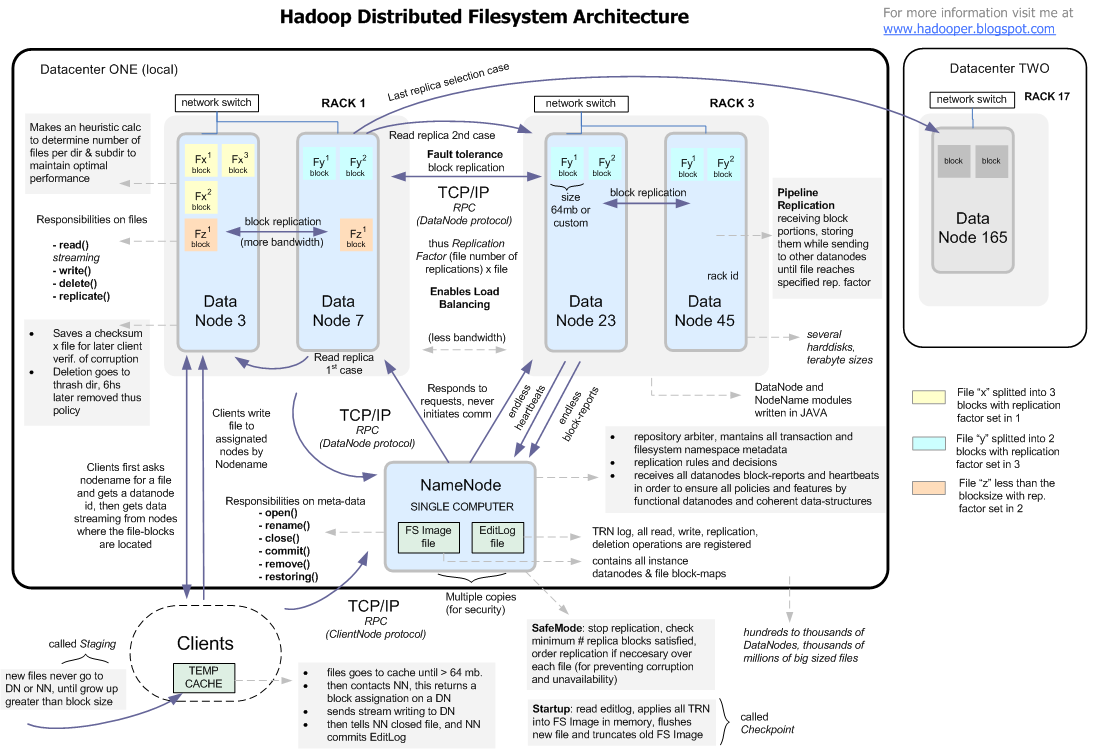
\includegraphics[scale=.33]{./img/HadoopDFSArchitecture.png}
\end{figure}


\section{Processing Model}
Main characteristics of Map Reduce   \\

\begin{itemize}
\item It's a processing model about dividing and distributing information, in two chained phases: map first, then reduce
\item Both phases have as input and output, a key-value pair list, 
\item The schema allows to define method parameters and own logic for both phases, as well as their own partitioning system and intermediate storage between phases.
\item The transactions are handled by a JobTracker daemon, that runs the initial data partitioning and the intermediate data combination, by posting tasks of type Map and type Reduce over the TaskTracker daemons (1-n x computer) of the nodes involved in the cluster, according the data being processed
\item The Reduce phase only starts when finished the Map, cause after the Map the resulting keys are combined, to distribute a sorted list of key-value pairs between the Reducers, that can be matched at the end of them.
\item The process is transactional, those map or reduce tasks not executed, (for data availability issues) will be reattempted a number of times, and then redistributed to other nodes.
\end{itemize}

\begin{figure}
\caption{The picture shows how these methods will interact in phases.}
\label{tab:hadoop_map_reduce_cycle}
\centering
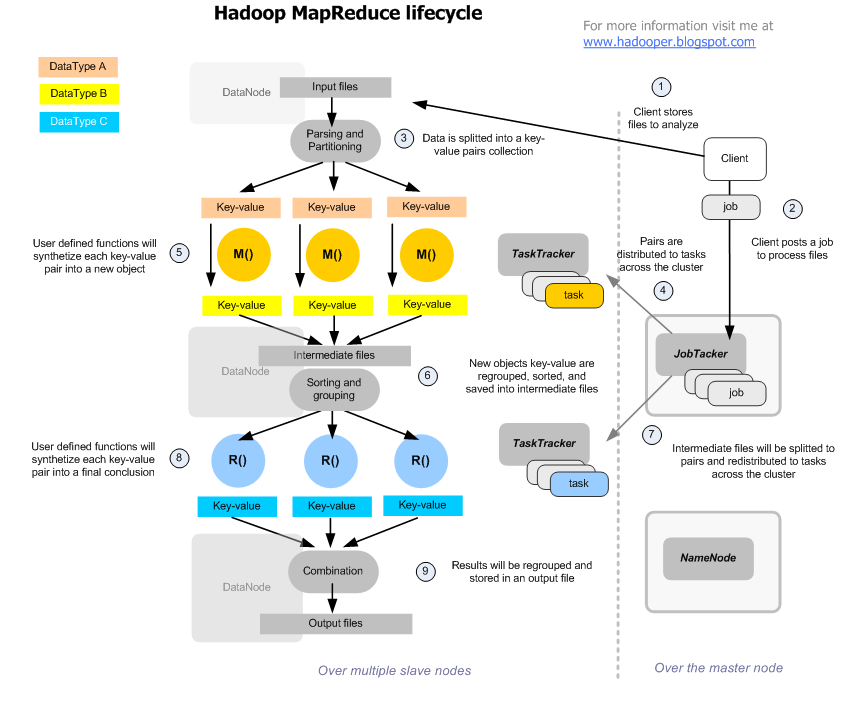
\includegraphics[scale=.33]{./img/HadoopMapReduceArchitecture.png}
\end{figure}

\begin{itemize}
\item First the files are partitioned in parts that will be distributed to process across the cluster nodes
\item  Each part is parsed in pairs of Key(sorteable object) - Value(object), that will be the input parameters for the tasks implementing the Map function
\item  These user defined tasks (map), will read the value object, do something with it, and then build a new key-value list that will be stored by the framework, in intermediate files.
\item  Once all the map tasks are finished, it means that the whole data to process was completely read, and reordered into this mapreduce model of key-value paris.
\item  These intermediate key-value results are combined, resulting a new paris of key-value that will be the input for the next reduce tasks
\item  These user defined tasks (reduce), will read the value object, do something with it, and then produce the 3rd and last list of key-value pairs, that the framework will combine, and regroup into a final result.

\end{itemize}
\begin{figure}
\caption{Let's see a sample job with a reverted-index function, for analyzing the webcrawler's output files (just for instance)}
\label{tab:hadoop_map_reduce_architecture}
\centering
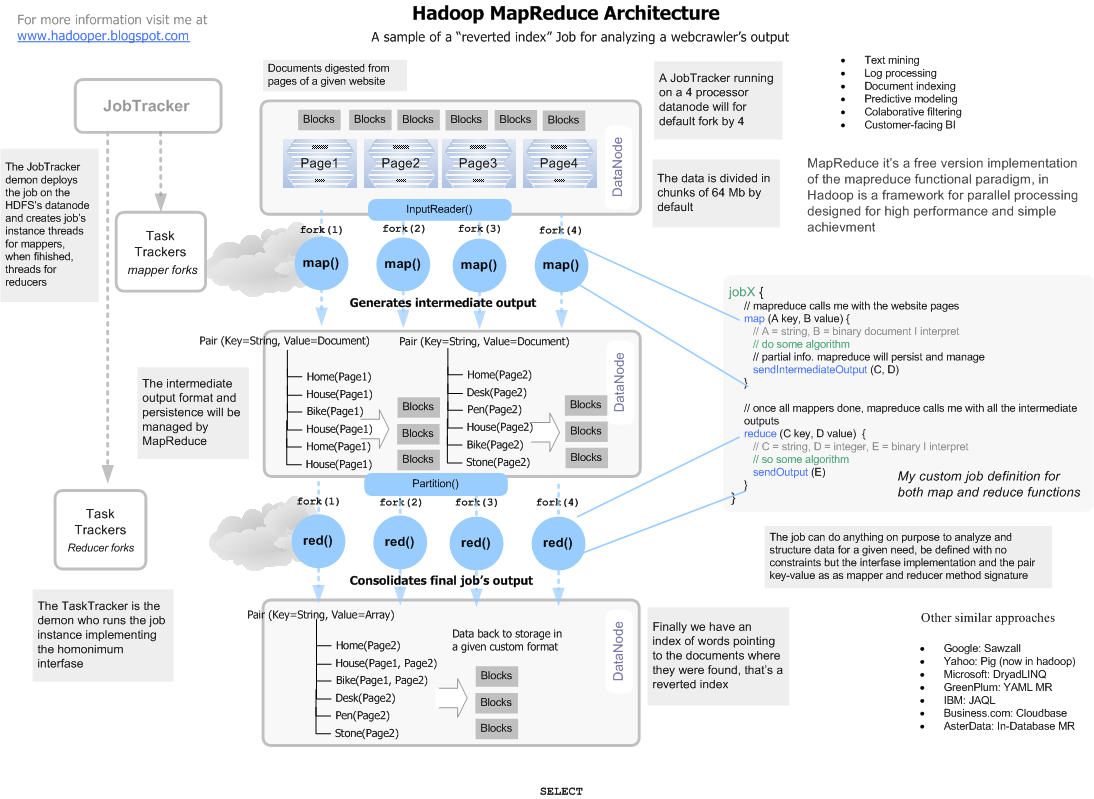
\includegraphics[scale=.33]{./img/HadoopMRProcessSample.png}
\end{figure}

MapReduce something, is about iterate a huge record collection, extract something good, mix and regroup intermediate results, that's all, it may look more complex than what it is.



%\part{Neural Network}
%%Relative path from root diectory
\documentclass[12pt, right open]{memoir}
\usepackage{graphicx}
\usepackage{tikz}
\usetikzlibrary{matrix,chains,positioning,decorations.pathreplacing,arrows,automata}
\usetikzlibrary{shapes.geometric, calc, intersections}
\usepackage{mathtools}
\usepackage{amsmath}
\usepackage{float}
\floatstyle{boxed}
\restylefloat{figure}

\usepackage{ifthen}
\setcounter{secnumdepth}{5}

\newcommand{\matplus}{
~~
  }

\begin{document}

%http://www.comp.leeds.ac.uk/ai23/reading/Hopfield.pdf

% >>>>>>>> Tikz Style sheet
\tikzstyle{every pin edge}=[<-,shorten <=1pt]
\tikzstyle{neuron}=[circle,fill=black!25,minimum size=17pt,inner sep=0pt]
\tikzstyle{input neuron}=[neuron, fill=black!50]
\tikzstyle{output neuron}=[neuron, fill=black!50]
\tikzstyle{hidden neuron}=[neuron, fill=black!50]
\tikzstyle{annot} = [text width=4em, text centered]

\tikzstyle{startstop} = [rectangle, rounded corners, minimum width=3cm, minimum height=1cm,text centered, draw=black]
\tikzstyle{io} = [trapezium, trapezium left angle=70, trapezium right angle=110, minimum width=3cm, minimum height=1cm, text centered, draw=black]
\tikzstyle{process} = [rectangle, minimum width=3cm, minimum height=1cm, text centered, text width=3cm, draw=black]
\tikzstyle{decision} = [diamond, minimum width=3cm, minimum height=1cm, text centered, draw=black]
\tikzstyle{arrow} = [thick,->,>=stealth]
% <<<<<<<< Tikz Style sheet

%%%%%%%%%%%%%%%%%%%%%%%%%%%%%%%%%%%%%%%%%%%%%%%%%%%%%%%%%%%%%%%%%%%%%%%%%%%%%%%%%%%%%%%%%%%
\chapter{What is Hopfield?}
\section{Introduction}

\def\layersep{2.5cm}
\begin{figure}[h!]
\caption{An artificial neuron as used in a Hopfield network} 
\label{fig:simple_hopfield_network}
\centering
\begin{tikzpicture}[shorten >=1pt,->,draw=black!50, node distance=\layersep]
    % Draw the input layer nodes
    \foreach \neuron in {1,...,3}
    % This is the same as writing \foreach \name / \y in {1/1,2/2,3/3,4/4}
        \node[input neuron] (I-\neuron) at (0,-\neuron) {\neuron};

    % Draw the output layer node
    \node[output neuron,pin={[pin edge={->}]right:Output}, right of=I-2] (O) {o};

    % Connect every node in the input layer with the output layer
    \foreach \source in {1,...,3}
        \path (I-\source) edge node[above] {$w_\source$} (O);

    % Annotate the layers
    \node[annot,below of=I-2] {Input layer};
    \node[annot,below of=O] {Output layer};

\end{tikzpicture}

\end{figure}

Hopfield networks are constructed from artificial neurons Figure~\ref{fig:simple_hopfield_network}. These
artificial neurons have N inputs. With each input $i$ there is a weight $w_i$ associated.
They also have an output. The state of the output is maintained, until
the neuron is updated. Updating the neuron entails the following operations:
	
\begin{itemize}
\item The value of each input, $x_i$ is determined and the weighted sum of all inputs,\(\vspace{2mm} \sum\limits_{i=1}^n {w_ix_i}\) is calculated.
\item The output state of the neuron is set to $+1$ if the weighted input sum is
larger or equal to $0$. It is set to $-1$ if the weighted input sum is smaller
than $0$.
\item A neuron retains its output state until it is updated again.
\end{itemize}

Written as formula: \\*
\[ o = \left\{ 
               \begin{array}{l l}
               \hspace{3 mm} 1  : & \quad \sum_{i} w_ix_i >= 0 \\
                            -1  : & \quad \sum_{i} w_ix_i < 0
               \end{array} 
       \right.
\]
  
  
A Hopfield network is a network of $N$ such artificial neurons, which are fully
connected. The connection weight from neuron $j$ to neuron $i$ is given by a
number $w$$_i$$_j$. The collection of all such numbers is represented by the weight
matrix $W$, whose components are $w$$_i$$_j$.

Now given the weight matrix and the updating rule for neurons the dynamics
of the network is defined if we tell in which order we update the neurons. There
are two ways of updating them:

\begin {itemize}
\item \textbf{Asynchronous}: one picks one neuron, calculates the weighted input sum
and updates immediately. This can be done in a fixed order, or neurons
can be picked at random, which is called asynchronous random updating.
\item \textbf{Synchronous}: the weighted input sums of all neurons are calculated without
updating the neurons. Then all neurons are set to their new value,
according to the value of their weighted input sum. The lecture slides
contain an explicit example of synchronous updating.
\end{itemize}

\section {Use of the Hopfield network}
The way in which the Hopfield network is used is as follows. 
A pattern is entered in the network by setting all nodes to a specific value, or by setting
only part of the nodes. The network is then subject to a number of iterations
using asynchronous or synchronous updating. This is stopped after a while.
The network neurons are then read out to see which pattern is in the network.
The idea behind the Hopfield network is that patterns are stored in the
weight matrix. The input must contain part of these patterns. The dynamics
of the network then retrieve the patterns stored in the weight matrix. This is
called \textbf{Content Addressable Memory (CAM)}. The network can also be used for
auto-association. The patterns that are stored in the network are divided in two
parts: \textbf{cue} and \textbf{association}. By entering the cue into the network,
the entire pattern, which is stored in the weight matrix, is retrieved. In this
way the network restores the association that belongs to a given cue.
The stage is now almost set for the Hopfield network, we must only decide
how we determine the weight matrix. We will do that in the next section, but
in general we always impose two conditions on the weight matrix:
\begin{itemize}
\item Symmetry : $w$$_i$$_j$ = $w$$_i$$_j$
\item No self connections: $w$$_i$$_i$ = 0
\end{itemize}

\begin{figure}
\centering
\caption{A two-neuron network}
\caption{There are just two options for the weight
matrix: $w_{i,j}$ = 1  or $w_{i,j}$ = -1. If the weight is 1, there are two stable
states under synchronous updating \{+1, +1\}, or \{-1, -1\}. For a weight of -1,
the stable states will be \{-1, +1\} or \{+1, -1\} depending on initial conditions.
Under synchrononous updating the states are oscillatory.}
\label{fig:a_two_neuron_network}
\begin{tikzpicture}[->,>=stealth,shorten >=1pt,auto,node distance=1cm,semithick]
    \node[input neuron] (N1) at (0,0) {1};
    \node[input neuron] (N2) at (4,0) {2};

    \path ([yshift= .5ex]N1.east) edge node[above] {$w_1$$_2$} ([yshift= .5ex]N2.west);
    \path ([yshift=-.5ex]N2.west) edge node[below] {$w_2$$_1$}([yshift=-.5ex]N1.east);
\end{tikzpicture}
\end{figure}

It turns out that we can guarantee that the network converges under asynchronous
updating when we use these conditions

\section{Training the network}
\subsection{A Simple Example}

Consider the two nodes in Fig~\ref{fig:a_two_neuron_network} Depending on which values they contain initially they will reach end states {+1, +1} or {-1,-1} under asynchronous
updating. \\
This simple example illustrates two important aspects of the Hopfield network:
the steady final state is determined by the value of the weight and the
network is ’sign-blind’; it depends on the initial conditions which final state will
be reached, \{+1,+1\} or \{-1, -1\} Figure~\ref{fig:a_two_neuron_network}.

\section{Setting the weight matrix}
\subsection{A single pattern}
Consider two neurons. If the weight between them is positive, then they will
tend to drive each other in the same direction: this is clear from the two-neuron
network in the example. It is also true in larger networks: suppose we have
neuron $i$ connected to neuron $j$ with a weight of $+1$, then the contribution of
neuron $i$ to the weighted input sum of neuron $j$ is \textbf{positive} if $x_i$ = $1$ and negative if $x = -1$. In other words neuron, $i$ tries to drive neuron $j$ to the same value as it has currently. If the connection weights between them is negative, however,
neuron $i$ will try to drive neuron $j$ to the opposite value! This inspires the
choice of the Hebb rule: given a network of N nodes and faced with a pattern
$~x = (x_1, ..., x_N )$ that we want to store in the network, we chose the values of
the weight matrix as follows:
\[ 
 w_{i,j} = x_ix_j
\]

\def\layersep{6cm}
\begin{figure}[h!]
\caption{Single Layer Hopfield network} 
\label{fig:single_layer_hopfield_network}
\centering

%\begin{tikzpicture}[shorten >=1pt,->,draw=black!50, node distance=\layersep, semithick]
\begin{tikzpicture}[->,>=stealth,shorten >=1pt,auto,node distance=1cm,semithick]
    % Draw the input layer nodes
    \node[input neuron] (N3) at (0,0) {3};
    \node[input neuron] (N1) at (0,4) {1};
    \node[input neuron] (N4) at (4,0) {4};
    \node[input neuron] (N2) at (4,4) {2};

    \path ([yshift= .5ex]N1.east) edge node[above] {-1} ([yshift= .5ex]N2.west);
    \path ([yshift=-.5ex]N2.west) edge node[below] {-1}([yshift=-.5ex]N1.east);
    
    \path ([xshift= .5ex]N2.south) edge node[right] {-1} ([xshift= .5ex]N4.north);
    \path ([xshift=-.5ex]N4.north) edge node[left] {-1}([xshift=-.5ex]N2.south);
    
    \path ([xshift= .5ex]N1.south) edge node[right] {1} ([xshift= .5ex]N3.north);
    \path ([xshift=-.5ex]N3.north) edge node[left] {1}([xshift=-.5ex]N1.south);
    
    \path ([yshift= .5ex]N3.east) edge node[above] {1} ([yshift= .5ex]N4.west);
    \path ([yshift=-.5ex]N4.west) edge node[below] {1}([yshift=-.5ex]N3.east); 
    
    \path ([xshift= 1ex]N1) edge node[right, pos =0.3] {1}([yshift= 1ex]N4.north west);
    \path ([xshift= 1ex]N4) edge node[left, pos =0.3] {1}([yshift=-1ex]N1.south east);

    \path ([xshift= 1ex]N3) edge node[left, pos =0.3] {-1}([yshift= 1ex]N2.south west);
    \path ([xshift= 1ex]N2) edge node[right, pos = 0.3] {-1}([yshift=-1ex]N3.north east);
        
\end{tikzpicture}
\end{figure}

To see how this works out in a network of four nodes, consider Figure~\ref{fig:a_two_neuron_network}. Note
that weights are optimal for this example in the sense that if the pattern (1, -1,
1, 1) is present in the network, each input node receives the maximal or minimal
(in the case of neuron 2) input some possible!
We can actually prove this: suppose the pattern $\vec{x}$, which has been used to
train the network, is present in the network and we update neuron i, what will
happen? The weighted input sum of a node is often denoted by $h_i = \sum_j w_{i,j}x_j$ ,
which is called the local field. If $w_{ij}$ was chosen to store this very same pattern,
we can calculate $h_i$:
\[
h_i = \sum_j w_{i,j}x_ix_j = \sum_{j=1}^3 = x_ix_jx_j = x_i + x_i + x_i = 3x_i 
\]

This is true for all nodes i. So all other three nodes (self connections are
forbidden!) in the network give a summed contribution of $3x_i$. This means that $x_i$ will never change value, the pattern is stable!

\[
h_i = \sum_j w_{i,j}v_j = - \sum_j w_{i,j}x_j = - \sum_j x_ix_jx_j = -\sum^3_{j=1} x_i = −3x_i = 3v_i
\]
Again, this pattern is maximally stable: the Hopfield network is ’sign-blind’.

\subsection{Weight Determination}
How to determine weight matrix for multiple patters? You can go about this in the following way.
\subsubsection{Binary to Bipolar Mapping}
By replacing each $0$ in a binary string with a $-1$, you get the corresponding bipolar string.
\[
f(x) = 2x - 1
\]
For inverse mapping, which turns a bipolar string into a binary string, you use
the following function:
\[
f(x) = (x + 1) / 2
\]
\subsubsection{Pattern’s Contribution to Weight}
We work with the bipolar versions of the input patterns. We take each
pattern to be recalled, one at a time, and determine its contribution to the
weight matrix of the network. The contribution of each pattern is itself a
matrix. The size of such a matrix is the same as the weight matrix of the
network. Then add these contributions, in the way matrices are added, and you
end up with the weight matrix for the network, which is also referred to as the
correlation matrix. Let us find the contribution of the pattern $A = (1, 0, 1, 0)$:
First, we notice that the binary to bipolar mapping of $A = (1, 0, 1, 0)$ gives the
vector $(1, –1, 1, –1)$.
Then we take the transpose, and multiply, the way matrices are multiplied, and
we see the following:

\[ 
\begin{bmatrix}
\matplus1  \\
-1  \\
\matplus1  \\
-1  \\
\end{bmatrix}
*
\begin{bmatrix}
 \matplus1 & -1 & \matplus1 & -1  \\
\end{bmatrix}
=
\begin{bmatrix}
 \matplus1 & -1 &  \matplus1 & -1 \\
-1 &  \matplus1 & -1 &  \matplus1 \\
 \matplus1 & -1 &  \matplus1 & -1 \\
-1 & \matplus1 & -1 &  \matplus1 \\
\end{bmatrix}
\]

Now subtract $1$ from each element in the main diagonal (that runs from top left
to bottom right). This operation gives the same result as subtracting the
identity matrix from the given matrix, obtaining $0$’s in the main diagonal. The
resulting matrix, which is given next, is the contribution of the pattern $(1, 0, 1,
0)$ to the weight matrix.
\[
 W_1 = \begin{bmatrix}
 \matplus0 & -1 &  \matplus1 & -1 \\
-1 &  \matplus0 & -1 &  \matplus1 \\
 \matplus1 & -1 &  \matplus0 & -1 \\
-1 &  \matplus1 & -1 &  \matplus0 \\
\end{bmatrix}
\]

Similarly, we can calculate the contribution from the pattern \\ $B = (0, 1, 0, 1)$ its bipolar version $B = (-1, 1, -1, 1)$ by verifying that pattern B's contribution is the same matrix as pattern A's contribution.

\[ 
\begin{bmatrix}
 -1  \\
  \matplus1  \\
 -1  \\
  \matplus1  \\
\end{bmatrix}
*
\begin{bmatrix}
 -1 & 1 & -1 & 1  \\
\end{bmatrix}
=
\begin{bmatrix}
 \matplus1 & -1 &  \matplus1 & -1 \\
-1 &  \matplus1 & -1 &  \matplus1 \\
 \matplus1 & -1 &  \matplus1 & -1 \\
-1 &  \matplus1 & -1 &  \matplus1 \\
\end{bmatrix}
\]
\[
W_2 =
\begin{bmatrix}
 \matplus0 & -1 &  \matplus1 & -1 \\
-1 &  \matplus0 & -1 &  \matplus1 \\
 \matplus1 & -1 &  \matplus0 & -1 \\
-1 &  \matplus1 & -1 &  \matplus0 \\
\end{bmatrix}
\]

\[
W_1 + W_2 =
\begin{bmatrix}
 \matplus0 & -2 &  \matplus2 & -2 \\
-2 &  \matplus0 & -2 &  \matplus2 \\
 \matplus1 & -2 &  \matplus0 & -2 \\
-2 &  \matplus1 & -2 &  \matplus0 \\
\end{bmatrix}
\]
We can now optionally apply an arbitrary scalar multiplier to all the entries of
the matrix if you wish. This is shown in the \ref{sec:example_a_simple_hopfield_network}.
\subsubsection{Autoassociative Network}
The Hopfield network just shown has the feature that the network associates an
input pattern with itself in recall. This makes the network an \textbf{autoassociative}
network. The patterns used for determining the proper weight matrix are also
the ones that are \textbf{autoassociatively} recalled. These patterns are called the
exemplars. A pattern other than an exemplar may or may not be recalled by the
network. Of course, when you present the pattern $0 0 0 0$, it is stable, even
though it is not an exemplar pattern.
\subsubsection{Orthogonal Bit Patterns}
You may be wondering how many patterns the network with four nodes is able
to recall. Let us first consider how many different bit patterns are orthogonal to
a given bit pattern. This question really refers to bit patterns in which at least
one bit is equal to 1. A little reflection tells us that if two bit patterns are to be
orthogonal, they cannot both have $1$'s in the same position, since the dot
product would need to be $0$. In other words, a bitwise logical $AND$ operation
of the two bit patterns has to result in a $0$. This suggests the following. If a
pattern $P$ has $k$, less than $4$, bit positions with $0$ (and so $4-k$ bit positions with
$1$), and if pattern $Q$ is to be orthogonal to $P$, then $Q$ can have $0$ or $1$ in those $k$ positions, but it must have only $0$ in the rest $4-k$ positions. Since there are two
choices for each of the $k$ positions, there are $2^k$ possible patterns orthogonal to
$P$. This number $2^k$ of patterns includes the pattern with all zeroes. So there
really are $2^k-1$ non-zero patterns orthogonal to $P$. Some of these $2^k-1$ patterns are not orthogonal to each other. As an example, $P$ can be the pattern (0 1 0 0),
which has $k=3$ positions with $0$. There are $2^3-1=7$ nonzero patterns
orthogonal to (0 1 0 0). Among these are patterns (1 0 1 0) and (1 0 0 1), which are
not orthogonal to each other, since their dot product is $1$ and not $0$.

\subsubsection{Network Nodes and Input Patterns}
Since our network has four neurons in it, it also has four nodes in the directed
graph that represents the network. These are laterally connected because
connections are established from node to node. They are lateral because the
nodes are all in the same layer. We started with the patterns A = (1, 0, 1, 0)
and B = (0, 1, 0, 1) as the exemplars. If we take any other nonzero pattern that
is orthogonal to A, it will have a 1 in a position where B also has a 1. So the
new pattern will not be orthogonal to B. Therefore, the orthogonal set of
patterns that contains A and B can have only those two as its elements. If you
remove B from the set, you can get (at most) two others to join A to form an
orthogonal set. They are the patterns (0, 1, 0, 0) and (0, 0, 0, 1).
If you follow the procedure described earlier to get the correlation matrix, you
will get the following weight matrix:


\[ 
W = \begin{bmatrix}
 \matplus0 & -1         &  \matplus3 & -1 \\
  -1       &  \matplus0 &  -1        &  -1 \\
 \matplus3 & -1         &  \matplus0 & -1 \\
-1         &  -1        & -1         &  \matplus0 \\
\end{bmatrix}
\]

With this matrix, pattern A is recalled, but the zero pattern (0, 0, 0, 0) is
obtained for the two patterns (0, 1, 0, 0) and (0, 0, 0, 1). Once the zero pattern
is obtained, its own recall will be stable.

\section{Energy}
We can define an energy for each node:
\[
E_i = - \frac{1}{2}h_ix_i
\]

Note that the energy is positive if the sign of $h_i$ and $x_i$
is different! An update of node i will result in a sign change in this case because the local field $h_i$ has a different sign. The updating will change the energy form a positive number
to a negative number. This corresponds to the intuitive idea that stable states
have a low energy. We can define an energy for the entire network:

\[
E(\vec{x}) = \sum_i E_i = - \sum_{i,j}\frac{1}{2}h_ix_i = -\frac{1}{2}\sum_{i,j}w_{i,j}x_ix_j
\]

Again, it is clear that for the pattern that has been used to train the weight
matrix the energy is minimal. In this case:

\[
E = -\frac{1}{2} \sum_{i,j}w_{i,j}x_ix_j = -\frac{1}{2} \sum_{i,j}x_ix_jx_j = -\frac{1}{2}
\sum_{i,j}1 = -\frac{1}{2}(N-1)^2
\]
\section{Stability of a single pattern}
So far we have looked at the situation where the same patterns was in the
network that was used to train the network. Now let us assume that another
pattern is in the network. It is pattern $\vec{y}$ which is the same as pattern $\vec{x}$ except for three nodes. The network, as usual, has $N$ nodes. No we are updating a
node $i$ of the network. What is the local field? It is given by:

\[
h_i = \sum_j w_{i,j}y_j = \sum_j x_ix_jy_j 
\]

We can split this sum in 3 nodes, which have an opposite value of $\vec{x}$ and
$N − 3$ nodes which have the same value:

\[
h_i = \sum^{N-3}_{j=1} x_ix_jx_j + \sum^3_{j=1} x_ix_j · -x_j = (N - 3)x_i - 3x_i = (N - 6)x_i
\]

For $N > 6$ all the local fields point the direction of $x_i$, the pattern that was
used to define the weight matrix!. So updating will result in no change (if the
value of node i is equal to $x_i$) or an update (if the value of node $i$ is equal to
$-x_i$). So, the pattern that is stored into the network is stable: up to half of the
nodes can be inverted and the network will still reproduce $\vec{x}$.

%There is also another way to look at this. The pattern that was used to train
%the network is an absolute energy minimum. This follows from equation 6. One
%can show the following important proposition, which is true for any symmetric
%weight matrix.
%
%Proposition 1:
%The energy of a Hopfield network can only decrease or stay the same. If an
%update cause a neuron to change sign, then the energy will decrease, otherwise
%it will stay the same.
%The condition that the energy of a Hopfield network can only decrease only rests
%on the condition that the weight matrix is symmetric. This is true for the Heb
%rule and also the generalised Hebb rule (see below). The undergraduates need
%not know this proof, but the postgraduates must be able to reproduce it. We
%will proof proposition 1 in section A.
%Since there is only one absolute minimum in a Hopfield network that has
%been trained with a single pattern (equation 6 is proof of that) and the minimum
%is reached when the training pattern (or its negative inverse; the same pattern
%with multiplied by -1) is in the network, the network must converge to the
%trained pattern (or its negative inverse).

%%%%%%%%%%%%%%%%%%%%%%%%%%%%%%%%%%%%%%%%%%%%%%%%%%%%%%%%%%%%%%%%%%%%%%%%%%%%%%%%%%%%%%%%%%%
\chapter{C++ Code}

\textbf{Code} :  aja/example/ann/hopfield\_network.cpp

\subsection {Example — A Simple Hopfield Network}
\label{sec:example_a_simple_hopfield_network}
A simple single layer Hopfield network is created with four neurons. We place, in
this layer, four neurons, each connected to the rest, as shown in Figure~\ref{fig:single_layer_hopfield_network}. Some of the connections have a positive weight, 
and the rest have a negative weight. The network
will be presented with two input patterns, one at a time, and it is supposed to recall them.
The inputs would be binary patterns having in each component a 0 or 1. If two patterns
of equal length are given and are treated as vectors, their dot product is obtained by first
multiplying corresponding components together and then adding these products. Two
vectors are said to be orthogonal, if their dot product is 0. The mathematics involved in
computations done for neural networks include matrix multiplication, transpose of a
matrix, and transpose of a vector. The inputs (which are stable, stored patterns) to be given should be orthogonal to one another.

\def\layersep{6cm}
\begin{figure}[h!]
\caption{Single Layer Hopfield network} 
\label{fig:single_layer_hopfield_network}
\centering

%\begin{tikzpicture}[shorten >=1pt,->,draw=black!50, node distance=\layersep, semithick]
\begin{tikzpicture}[->,>=stealth,shorten >=1pt,auto,node distance=1cm,semithick]
    % Draw the input layer nodes
    \node[input neuron] (N3) at (0,0) {3};
    \node[input neuron] (N1) at (0,4) {1};
    \node[input neuron] (N4) at (4,0) {4};
    \node[input neuron] (N2) at (4,4) {2};

    \path ([yshift= .5ex]N1.east) edge node[above] {$w_1$$_2$} ([yshift= .5ex]N2.west);
    \path ([yshift=-.5ex]N2.west) edge node[below] {$w_2$$_1$}([yshift=-.5ex]N1.east);
    
    \path ([xshift= .5ex]N2.south) edge node[right] {$w_2$$_4$} ([xshift= .5ex]N4.north);
    \path ([xshift=-.5ex]N4.north) edge node[left] {$w_4$$_2$}([xshift=-.5ex]N2.south);
    
    \path ([xshift= .5ex]N1.south) edge node[right] {$w_1$$_3$} ([xshift= .5ex]N3.north);
    \path ([xshift=-.5ex]N3.north) edge node[left] {$w_3$$_1$}([xshift=-.5ex]N1.south);
    
    \path ([yshift= .5ex]N3.east) edge node[above] {$w_3$$_4$} ([yshift= .5ex]N4.west);
    \path ([yshift=-.5ex]N4.west) edge node[below] {$w_4$$_3$}([yshift=-.5ex]N3.east); 
    
    \path ([xshift= 1ex]N1) edge node[right, pos =0.3] {$w_1$$_4$}([yshift= 1ex]N4.north west);
    \path ([xshift= 1ex]N4) edge node[left, pos =0.3] {$w_4$$_1$}([yshift=-1ex]N1.south east);

    \path ([xshift= 1ex]N3) edge node[left, pos =0.3] {$w_3$$_2$}([yshift= 1ex]N2.south west);
    \path ([xshift= 1ex]N2) edge node[right, pos = 0.3] {$w_2$$_3$}([yshift=-1ex]N3.north east);
        
\end{tikzpicture}
\end{figure}

The two patterns we want the network to recall are $A = (1, 0, 1, 0)$ and $B = (0, 1, 0, 1)$,
which you can verify to be orthogonal. Recall that two vectors A and B are orthogonal if
their dot product is equal to zero. This is true in this case since

$A_1$$B_1$ + $A_2$$B_2$ + $A_3$$B_3$ + $A_4$$B_4$ = $(1\times0 + 0\times1 + 1\times0 + 0\times1) = 0$

The following matrix W gives the weights on the connections in the network.

\[ 
W = \begin{bmatrix}
 \matplus0 & -3 &  \matplus3 & -3 \\
-3 &  \matplus0 & -3 &  \matplus3 \\
 \matplus3 & -3 &  \matplus0 & -3 \\
-3 &  \matplus3 & -3 &  \matplus0 \\
\end{bmatrix}
\]

We need a threshold function also, and we define it as follows. The threshold value $\theta$ is 0.

\[ f(t) = \left\{ 
                  \begin{array}{l l}
                   1 & \mbox{if $t \geq \theta$}\\
                   0 & \mbox{if $t < \theta$}
                  \end{array} 
          \right. 
\]
 
 
 We have four neurons in the only layer in this network. We need to compute
the activation of each neuron as the weighted sum of its inputs. The activation
at the first node is the dot product of the input vector and the first column of
the weight matrix (0 -3 3 -3). We get the activation at the other nodes
similarly. The output of a neuron is then calculated by evaluating the threshold
function at the activation of the neuron. So if we present the input vector A,
the dot product works out to 3 and f(3) = 1. Similarly, we get the dot products
of the second, third, and fourth nodes to be -6, 3, and -6, respectively. The
corresponding outputs therefore are 0, 1, and 0. This means that the output of
the network is the vector (1, 0, 1, 0), same as the input pattern. The network
has recalled the pattern as presented, or we can say that pattern A is stable,
since the output is equal to the input. When B is presented, the dot product
obtained at the first node is -6 and the output is 0. The outputs for the rest of
the nodes taken together with the output of the first node gives (0, 1, 0, 1),
which means that the network has stable recall for B also.

So far we have presented easy cases to the network—vectors that the Hopfield
network was specifically designed (through the choice of the weight matrix) to
recall. What will the network give as output if we present a pattern different
from both A and B? Let C = (0, 1, 0, 0) be presented to the network. The
activations would be -3, 0, -3, 3, making the outputs 0, 1, 0, 1, which means
that B achieves stable recall. This is quite interesting. Suppose we did intend to
input B and we made a slight error and ended up presenting C, instead. The
network did what we wanted and recalled B. But why not A? To answer this,
let us ask is C closer to A or B? How do we compare? We use the distance
formula for two four-dimensional points. If (a, b, c, d) and (e, f, g, h) are two
four-dimensional points, the distance between them is:

\[\sqrt{(a – e)^2 + (b – f)^2 + (c – g)^2 + (d – h)^2}\]

The distance between A and C is $\sqrt{3}$, whereas the distance between B and
C is just 1. So since B is closer in this sense, B was recalled rather than A. You
may verify that if we do the same exercise with D = (0, 0, 1, 0), we will see
that the network recalls A, which is closer than B to D.


\section{Asynchronous Update}

The Hopfield network is a recurrent network. This means that outputs from
the network are fed back as inputs. This is not apparent from Figure\ref{fig:asynchonous_update_flow}.

The Hopfield network always stabilizes to a fixed point. There is a very
important detail regarding the Hopfield network to achieve this stability. In the
examples thus far, we have not had a problem getting a stable output from the
network, so we have not presented this detail of network operation. This detail
is the need to update the network asynchronously. This means that changes do
not occur simultaneously to outputs that are fed back as inputs, but rather
occur for one vector component at a time.

\begin{figure}[!ht] %Create figure holder
\caption{Asynchonous Update Flow}
\label{fig:asynchonous_update_flow}
\centering
\begin{tikzpicture}[node distance=2cm] %use the ‘tikzpicture’ environment

%      node_var  style   display text
\node (start) [startstop] {Start};
\node (input) [io, below of=start] {Inputs};
\node (hopfield_network) [process, below of=input] {Hopfield Network};
\node (update) [process, left of=hopfield_network, xshift=-2cm] {Update};
\node (threshold_function) [process, below of=hopfield_network] {Threshold Function};
\node (output) [io, below of=threshold_function] {Output};
\node (stop) [startstop, below of=output] {Stop};
%
\draw [arrow] (start) -- (input);
\draw [arrow] (input) -- (hopfield_network);
\draw [arrow] (hopfield_network) -- (threshold_function);
\draw [arrow] (threshold_function) -- (output);
\draw [arrow] (output) -- (stop);

\draw [arrow] (output) -|  (update);
\draw [arrow] (update) |- (input);

\end{tikzpicture}
\end{figure}

The true operation of the Hopfield network follows the procedure below for input vector \textbf{Invec} and output vector \textbf{Outvec}:

\begin {itemize}
\item Apply an input, Invec, to the network, and initialize Outvec = Invec
\item Start with i = 1
\item Calculate Value i = DotProduct ( Invec i, Column i of Weight matrix)4. 
\item Calculate Outvec i = f(Value i ) where f is the threshold function discussed previously
\item Update the input to the network with component Outvec i
\item Increment i, and repeat steps 3, 4, 5, and 6 until Invec = Outvec(note that when i reaches its maximum value, it is then next reset to 1 for the cycle to continue)
\end{itemize}

Now let’s see how to apply this procedure. Building on the last example, we
now input E = (1, 0, 0, 1), which is at an equal distance from A and B. Without
applying the asynchronous procedure above, but instead using the shortcut
procedure we’ve been using so far, you would get an output F = (0, 1, 1, 0).
This vector, F, as subsequent input would result in E as the output. This is
incorrect since the network oscillates between two states. We have updated the
entire input vector synchronously.
Now let’s apply asynchronous update. For input E, (1,0,0,1) we arrive at the
following results detailed for each update step, in Table \ref{tab:example_of_asynchronous_update_for_the_hopfield_network}

\begin{center}
\begin{table}
\caption{Example of Asynchronous Update for the Hopfield Network}
\label{tab:example_of_asynchronous_update_for_the_hopfield_network}
\begin{tabular}{|l|l|l|p{3cm}|l|l|p{3cm}|}
\hline
Step & i & Invec & Column of weight vectors & Value & Outvec & notes \\
\hline
0    &   & 1001  &                          &       & 1001   & initialization : set Outvec = Invec =Input pattern\\
\hline
1    & 1 & 1001  & 0 -3 3 -3                & -3    & 0001   & column 1 of Outvec
changed to 0\\
\hline
2    & 2 & 0001  & -3 0 -3 3                &  3    & 0101   & column 2 of Outvec
changed to 1\\
\hline
3    & 3 & 0101  & 3 -3 0 -3                & -6    & 0101   & column 3 of Outvec
stays as 0\\
\hline
4    & 4 & 0101  & -3 3 -3 0                &  3    & 0101   & column 4 of Outvec
stays as 1\\
\hline
5    & 1 & 0101  & 0 -3 3 -3                & -6    & 0101   & column 1 stable as 0\\
\hline
6    & 2 & 0101  & -3 0 -3 3                &  3    & 0101   & column 2 stable as 1\\
\hline
7    & 3 & 0101  & 3 -3 0 -3                & -6    & 0101   & column 3 stable as 0\\
\hline
8    & 4 & 0101  & -3 3 -3 0                &  3    & 0101   & column 4 stable as
1; stable recalled pattern = 0101\\
\hline
\end{tabular}
\end{table}
\end{center}

\section{Classes in C++ Implementation}
In our C++ implementation of this network, there are the following classes: a
\textbf{network class}, and a \textbf{neuron class}. In our implementation, we create the
network with four neurons, and these four neurons are all connected to one
another. A neuron is not self-connected, though. That is, there is no edge in the
directed graph representing the network, where the edge is from one node to
itself. But for simplicity, we could pretend that such a connection exists
carrying a weight of 0, so that the weight matrix has 0’s in its principal
diagonal.

The functions that determine the neuron activations and the network output are
declared public. Therefore they are visible and accessible without restriction.
The activations of the neurons are calculated with functions defined in theneuron class. When there are more than one layer in a neural network, the
outputs of neurons in one layer become the inputs for neurons in the next
layer. In order to facilitate passing the outputs from one layer as inputs to
another layer, our C++ implementations compute the neuron outputs in the
network class. For this reason the threshold function is made a member of the
network class. We do this for the Hopfield network as well. To see if the
network has achieved correct recall, you make comparisons between the
presented pattern and the network output, component by component.

\section{A New Weight Matrix to Recall More Patterns}
Let’s continue to discuss this example. Suppose we are interested in having the
patterns $E = (1, 0, 0, 1)$ and $F = (0, 1, 1, 0)$ also recalled correctly, in addition
to the patterns $\vec{A}$ and $\vec{B}$. In this case we would need to train the network and
come up with a learning algorithm, which we will discuss in more detail later
in the book. We come up with the matrix $W_1$, which follows...
\[ 
W_1 = \begin{bmatrix}
 \matplus0 & -5 &  \matplus4 & \matplus4 \\
-5 &  \matplus0 &  \matplus4 & \matplus4 \\
 \matplus4 &  \matplus4 &  \matplus0 & -5 \\
 \matplus4 &  \matplus4 & -5 &  \matplus0 \\
\end{bmatrix}
\]
Try to use this modification of the weight matrix in the source program, and
then compile and run the program to see that the network successfully recalls
all four patterns A, B, E, and F.

%%%%%%%%%%%%%%%%%%%%%%%%%%%%%%%%%%%%%%%%%%%%%%%%%%%%%%%%%%%%%%%%%%%%%%%%%%%%%%%%%%%%%%%%%%%
\end{document}

%Frequently update this section from aja/docs/latex_tutorial/latex_template.tex
%To get all latest inclusion updates on book seetings.

%TODO: This should be made as book template for aja use!
%memoir  is the book template from LaTeX
\documentclass[12pt, right open]{memoir}
%To draw stuff on out documents
\usepackage{graphicx}
\usepackage{tikz}
\usepackage{xcolor}
%indivudual library needed on ad-hoc basis
\usetikzlibrary{matrix,chains,positioning,decorations.pathreplacing,arrows,automata}
%To perform coordinate calculations, the calc library is required,
%calculations are enclosed in $
\usetikzlibrary{shapes.geometric, calc, intersections}
%Maths tools
\usepackage{mathtools}
\usepackage{amsmath}
\usepackage{float}
\floatstyle{boxed}
\restylefloat{figure}
\usepackage{multirow} %for tables
\usepackage{ifthen}
%http://en.wikibooks.org/wiki/LaTeX/Algorithms
\usepackage{algorithmic}
\setcounter{secnumdepth}{5}

%To reduce vetical line spaces between list items
\usepackage{enumitem}
\setlist{nolistsep,leftmargin=*}

\newcommand{\specialcell}[2][c]{%
  \begin{tabular}[#1]{@{}c@{}}#2\end{tabular}}
%  Foo bar & \specialcell{Foo\\bar} & Foo bar \\    % vertically centered
%Foo bar & \specialcell[t]{Foo\\bar} & Foo bar \\ % aligned with top rule
%Foo bar & \specialcell[b]{Foo\\bar} & Foo bar \\ % aligned with bottom rule

%to tackle spaces in -1 n +1
\newcommand{\matplus}{
~~
  }

%For listing code
\usepackage{listings}
\usepackage{xcolor} % for setting colors

% set the default code style
\lstset{
    frame=tb, % draw a frame at the top and bottom of the code block
    tabsize=4, % tab space width
    showstringspaces=false, % don't mark spaces in strings
 %   numbers=left, % display line numbers on the left
    commentstyle=\color{green}, % comment color
    keywordstyle=\color{blue}, % keyword color
    stringstyle=\color{red} % string color
    breaklines=true,
}

\lstdefinestyle{codeTex}{
  belowcaptionskip=1\baselineskip,
  breaklines=true,
  frame=L,
  xleftmargin=\parindent,
  language=Tex,
  showstringspaces=false,
  basicstyle=\footnotesize\ttfamily,
  keywordstyle=\bfseries\color{green!40!black},
  commentstyle=\itshape\color{purple!40!black},
  identifierstyle=\color{blue},
  stringstyle=\color{orange},
}

\lstdefinestyle{codeC}{
  belowcaptionskip=1\baselineskip,
  breaklines=true,
  frame=L,
  xleftmargin=\parindent,
  language=C,
  showstringspaces=false,
  basicstyle=\footnotesize\ttfamily,
  keywordstyle=\bfseries\color{green!40!black},
  commentstyle=\itshape\color{purple!40!black},
  identifierstyle=\color{blue},
  stringstyle=\color{orange},
}
%\begin{lstlisting}[style=codeC]
%---------------
%\end{lstlisting}
%\lstinputlisting[caption=Scheduler, style=customc]{hello.c}


\begin{document}

%http://www.comp.leeds.ac.uk/ai23/reading/Hopfield.pdf

%TODO: Needs to find an easy way to draw neural nets

% >>>>>>>> Tikz Style sheet
% Create Tikz style, something like typedef in C, where we can specify the shape, color, size, text details etc

\tikzstyle{every pin edge}=[<-,shorten <=1pt]
\tikzstyle{neuron}=[circle,fill=black!10,minimum size=25pt,inner sep=0pt]
\tikzstyle{input neuron}=[neuron, fill=black!40]
\tikzstyle{output neuron}=[neuron, fill=black!40]
\tikzstyle{hidden neuron}=[neuron, fill=black!10]
\tikzstyle{annot} = [text width=4em, text centered]

\tikzstyle{startstop} = [rectangle, rounded corners, minimum width=3cm, minimum height=1cm,text centered, draw=black, fill=red!30]
\tikzstyle{io} = [trapezium, trapezium left angle=70, trapezium right angle=110, minimum width=3cm, minimum height=1cm, text centered, draw=black, fill=blue!30]
%\tikzstyle{process} = [rectangle, minimum width=3cm, minimum height=1cm, text centered, draw=black, fill=orange!30]
\tikzstyle{process} = [rectangle, minimum width=3cm, minimum height=1cm, text centered, text width=3cm, draw=black, fill=orange!30]
\tikzstyle{decision} = [diamond, minimum width=3cm, minimum height=1cm, text centered, draw=black, fill=green!30]
\tikzstyle{arrow} = [thick,->,>=stealth]
% <<<<<<<< Tikz Style sheet

%%%%%%%%%%%%%%%%%%%%%%%%%%%%%%%%%%%%%%%%%%%%%%%%%%%%%%%%%%%%%%%%%%%%%%%%%%%%%%%%%%%%%%%%%%%
\chapter{Backpropagation}

\section{Feedforward Backpropagation Network}
The feedforward backpropagation network is a \textbf{very popular model} in neural
networks. It \textbf{does not have feedback connections}, but errors are
backpropagated during training. \textbf{Least mean squared error} is used. Many
applications can be formulated for using a feedforward backpropagation
network, and the methodology has been a model for most multilayer neural
networks. Errors in the output determine measures of hidden layer output
errors, which are used as a basis for adjustment of connection weights between
the input and hidden layers. Adjusting the two sets of weights between the
pairs of layers and recalculating the outputs is an iterative process that is
carried on until the errors fall below a tolerance level. Learning rate
parameters scale the adjustments to weights. A momentum parameter can also
be used in scaling the adjustments from a previous iteration and adding to the
adjustments in the current iteration.

\subsection{Mapping}
The feedforward backpropagation network maps the input vectors to output
vectors. Pairs of input and output vectors are chosen to train the network first.
Once training is completed, the weights are set and the network can be used to
find outputs for new inputs. The \textbf{dimension of the input vector determines} the
\textbf{number of neurons in the input layer}, and the \textbf{number of neurons in the output
layer} is determined by the \textbf{dimension of the outputs}. If there are $k$ neurons in
the input layer and $m$ neurons in the output layer, then this network can make a
mapping from $k$-dimensional space to an $m$-dimensional space. Of course,
what that mapping is depends on what pair of patterns or vectors are used as 
exemplars to train the network, which determine the network weights. Once
trained, the network gives you the image of a new input vector under this
mapping. Knowing what mapping you want the feedforward backpropagation
network to be trained for implies the dimensions of the input space and the
output space, so that you can determine the numbers of neurons to have in the
input and output layers.

\subsection{Layers}

The architecture of a feedforward backpropagation network is shown in Figure \ref{fig:simple_backpropagation}. While there can be many hidden layers, we will illustrate this network with only one hidden layer. Also, the number of neurons in the input layer and
that in the output layer are determined by the dimensions of the input and
output patterns, respectively. It is not easy to determine how many neurons are
needed for the hidden layer. In order to avoid cluttering the figure, we will
show the layout in Figure \ref{fig:simple_backpropagation} with four input neurons, three neurons in the
hidden layer, and one output neuron(s), with a few representative connections.
The network has three fields of neurons: one for input neurons, one for hidden
processing elements, and one for the output neurons. As already stated,
connections are for feed forward activity. There are connections from every
neuron in field A to every one in field B, and, in turn, from every neuron in
field B to every neuron in field C. Thus, there are two sets of weights, those
figuring in the activations of hidden layer neurons, and those that help
determine the output neuron activations. In training, all of these weights are
adjusted by considering what can be called a cost function in terms of the error
in the computed output pattern and the desired output pattern.

\def\layersep{2.5cm}
\begin{figure}[ht!]
\caption{An simple Backpropagation Network} 
\label{fig:simple_backpropagation}
\centering
\begin{tikzpicture}[shorten >=1pt,->,draw=black!50, node distance=\layersep]
    % Draw the input layer nodes
    \foreach \neuron in {1,...,3}
    % This is the same as writing \foreach \name / \y in {1/1,2/2,3/3,4/4}
    \node[input neuron] (I-\neuron) at (0,-\neuron-0.5) {\neuron};
    
    \foreach \neuron in {1,...,4}
    % This is the same as writing \foreach \name / \y in {1/1,2/2,3/3,4/4}
    \node[hidden neuron, right of=I-0] (H-\neuron) at (0,-\neuron) {\neuron};

    % Draw the output layer node
    \node[output neuron,pin={[pin edge={->}]right:Output}, right of=H-2] (Output) {o};

    % Connect every node in the input layer with the output layer
    \foreach \InputLayerNeuron in {1,...,3}
    	\foreach \HiddenLayerNeuron in {1,...,4}
    	        	%edge node[above] {$w_{\HiddenLayerNeuron\InputLayerNeuron}$}
        	\path (I-\InputLayerNeuron)  edge (H-\HiddenLayerNeuron);

     \foreach \HiddenLayerNeuron in {1,...,4}
     	\path (H-\HiddenLayerNeuron) edge node[above]{$w_{o\HiddenLayerNeuron}$} (Output);
    % Annotate the layers
    \node[annot,below of=I-2] {Input layer};
    \node[annot,below of=Output] {Output layer};
\end{tikzpicture}
\end{figure}

\section{Training}

The feedforward backpropagation network undergoes supervised training, with
a finite number of pattern pairs consisting of an input pattern and a desired or
target output pattern. An input pattern is presented at the input layer. The
neurons here pass the pattern activations to the next layer neurons, which are
in a hidden layer. The outputs of the hidden layer neurons are obtained by
using perhaps a \textbf{bias}, and also a threshold function with the activations
determined by the weights and the inputs. These hidden layer outputs become
inputs to the output neurons, which process the inputs using an optional bias
and a threshold function. The final output of the network is determined by the
activations from the output layer.
The computed pattern and the input pattern are compared, a function of this
error for each component of the pattern is determined, and adjustment to
weights of connections between the \textbf{hidden layer} and \textbf{the output layer} is
computed. A similar computation, still based on the error in the output, is
made for the connection weights between the \textbf{input} and \textbf{hidden layers}. The
procedure is repeated with each pattern pair assigned for training the network.Each pass through all the training patterns is called a \textbf{cycle or an epoch}. The
process is then repeated as many cycles as needed until the error is within a
prescribed tolerance.

\section{Illustration}
\subsection{Adjustment of Weights of Connections from a Neuron in
the Hidden Layer}

We will be as specific as is needed to make the computations clear. First recall that the activation of a neuron in a layer other than the input layer is the sum of products of its inputs and the weights corresponding to the connections that bring in those inputs. Let us discuss the $j$th neuron in the hidden layer. Let us be specific and say $j = 2$. Suppose that the input pattern is $(1.1, 2.4, 3.2, 5.1, 3.9)$ and the target output pattern is $(0.52, 0.25, 0.75, 0.97)$. Let the weights be given for the second hidden layer
neuron by the vector $(-0.33, 0.07, -0.45, 0.13, 0.37)$. The activation will be the quantity:\\

$(-0.33 * 1.1) + (0.07 * 2.4) + (-0.45 * 3.2) + (0.13 * 5.1)
+ (0.37 * 3.9) = 0.471$\\

Now add to this an optional bias of, say, $0.679$, to give $1.15$. 
If we use the sigmoid function given by:
\[
 \frac{1}{1+\exp{^{-x}}}
\]
with x = 1.15, we get the output of this hidden layer neuron as $0.7595$.\\

We need the computed output pattern also. Let us say it turns out to be $actual = (0.61, 0.41, 0.57, 0.53)$, while the desired pattern is $desired = (0.52, 0.25, 0.75, 0.97)$. Obviously, there is a discrepancy between what is desired and what is computed. The component-wise differences are given in the vector, $desired - actual = (-0.09, -0.16, 0.18, 0.44)$.\\

We use these to form another vector where each component is a product of the error component, corresponding computed pattern component, and the complement of the latter with respect to 1. For example, for the first component, error is $-0.09$, computed pattern component is 0.61, and its complement is 0.39. Multiplying these together $(0.61*0.39*-0.09)$, we get $-0.02$. Calculating the other components similarly, we get the vector $(-0.02, -0.04, 0.04, 0.11)$.  i.e  error = $actual \times (1 - actual) \times (d - a)$ \\

The $desired-actual$ vector, which is the error vector multiplied by the actual output vector, gives you a value of error reflected back at the output of the hidden layer. This is scaled by a value of (1-output vector), which is the first derivative of the output activation function for numerical stability). You will see the
formulas for this process later in this chapter. The backpropagation of errors needs to be carried further. We need now the weights on the connections between the second neuron in the hidden layer that we are concentrating on, and the different output neurons. Let us say these weights are given by the vector $(0.85, 0.62, –0.10, 0.21)$. The error of the second neuron in the hidden layer is now calculated as below, using its output.\\

$error = 0.7595 * (1 - 0.7595) * ( (0.85 * -0.02) + (0.62 * -0.04)
+ ( -0.10 * 0.04) + (0.21 * 0.11)) = -0.0041.$\\

Again, here we multiply the error $(e.g., -0.02)$ from the output of the current layer, by the output value $(0.7595)$ and the value $(1-0.7595)$. We use the weights on the connections between neurons to work backwards through the network. Next, we need the learning rate parameter for this layer; let us set it as $0.2$. We multiply this by the output of the second neuron in the hidden layer, to get $0.1519$. Each of the components of the vector $(-0.02, -0.04, 0.04, 0.11)$ is multiplied now by $0.1519$, which our latest computation gave. The result is a vector that gives the adjustments to the weights on the connections that go from the second neuron in the hidden layer to the output neurons. These values are given in the vector $(-0.003, -0.006, 0.006,0.017)$. After these adjustments are added, the weights to be used in the next cycle on the connections between the second neuron in the hidden layer and the output neurons become those in the vector
$(0.847, 0.614, -0.094, 0.227)$.

\subsection{Adjustment of Weights of Connections from a Neuron in
the Input Layer}

Let us look at how adjustments are calculated for the weights on connections going from the ith neuron in the input layer to neurons in the hidden layer. Let us take specifically i = 3, for illustration. Much of the information we need is already obtained in the previous discussion for the second hidden layer neuron. We have the errors in the computed output as the vector (–0.09, –0.16, 0.18, 0.44), and we obtained the error for the second neuron in the hidden layer as –0.0041, which was not used above. Just as the error in the output is propagated back to assign errors for the neurons in the hidden layer, those errors can be propagated to the input layer neurons.
To determine the adjustments for the weights on connections between the input and hidden layers, we need the errors determined for the outputs of hidden layer neurons, a learning rate parameter, and the activations of the input neurons, which are just the input values for the input layer. Let us take the learning rate parameter to be 0.15. Then the weight adjustments for the connections from the third input neuron to the hidden layer neurons are obtained by multiplying the particular hidden layer neuron’s output error by the learning rate parameter and by the input component from the input neuron. The adjustment for the weight on the connection from the third input neuron to the second hidden layer neuron is 0.15 * 3.2 * –0.0041, which works out to –0.002. If the weight on this connection is, say, –0.45, then adding the adjustment of -0.002, we get the modified
weight of –0.452, to be used in the next iteration of the network operation. Similar calculations are made to modify all other weights as well.

\subsection{Adjustments to Threshold Values or Biases}
The bias or the threshold value we added to the activation, before applying the
threshold function to get the output of a neuron, will also be adjusted based on
the error being propagated back. The needed values for this are in the previous
discussion.
The adjustment for the threshold value of a neuron in the output layer is
obtained by multiplying the calculated error (not just the difference) in the
output at the output neuron and the learning rate parameter used in the
adjustment calculation for weights at this layer. In our previous example, we
have the learning rate parameter as 0.2, and the error vector as (–0.02, –0.04,
0.04, 0.11), so the adjustments to the threshold values of the four output
neurons are given by the vector (–0.004, –0.008, 0.008, 0.022). These
adjustments are added to the current levels of threshold values at the output
neurons.
The adjustment to the threshold value of a neuron in the hidden layer is
obtained similarly by multiplying the learning rate with the computed error in
the output of the hidden layer neuron. Therefore, for the second neuron in the
hidden layer, the adjustment to its threshold value is calculated as 0.15 *
–0.0041, which is –0.0006. Add this to the current threshold value of 0.679 to
get 0.6784, which is to be used for this neuron in the next training pattern for
the neural network.

\section{Mathematical Derivations}

\begin{itemize}

\item Uses Delta learning rule

\begin{align*}
\Delta w = \eta r x \\
rx = \Delta E \\
\Delta w = - \eta \Delta E \\
\end{align*}

\item It follows gradient descent method

\def\layersep{3.5cm}
\begin{figure}[ht!]
\caption{An Multi Layer Backpropagation Network} 
\label{fig:an_multi_layer_backpropagation}
\centering
\begin{tikzpicture}[shorten >=1pt,->,draw=black!20, node distance=\layersep]
    % Draw the input layer neurons
    \node[input neuron] (I-1) at (0,-1) {$x_1$};
    \node[input neuron] (I-2) at (0,-2) {$x_i$};
    \node[input neuron] (I-3) at (0,-3) {$x_n$};
    
    % Draw the hidden layer neurons
    \node[hidden neuron] (H-1) at (2,-1) {$z_1$};
    \node[hidden neuron] (H-2) at (2,-2) {$z_j$};
    \node[hidden neuron] (H-3) at (2,-3) {$z_p$};
    
    \node[hidden neuron] (B-0) at (.5,-4) {$x_0$};

    \node[output neuron] (O-1) at (4, -1) {$y_1$};
    \node[output neuron] (O-2) at (4, -2) {$y_k$};
    \node[output neuron] (O-3) at (4, -3) {$y_m$};
    
    \node[hidden neuron] (B-1) at (2.5,-4) {$z_0$};

    % Connect every node in the input layer with the output layer
    \foreach \InputLayerNeuron in {1,...,3}
    	\foreach \HiddenLayerNeuron in {1,...,3}
        	\path (I-\InputLayerNeuron)  edge (H-\HiddenLayerNeuron);	

     \foreach \HiddenLayerNeuron in {1,...,3}
     \foreach \OutputLayerNeuron in {1,...,3}
        	\path (H-\HiddenLayerNeuron)  edge (O-\OutputLayerNeuron);
        	
     %\node[output neuron,pin={[pin edge={->}]right:Output}, right of=I-2] (Output) {o};
     \draw[thick, ->] (O-2) -- (6, -2) node[above] {$O_{jk}$} ;
     % Connect every node in the input layer with the output layer
    \foreach \HiddenLayerNeuron in {1,...,3}
    		\path (B-0)  edge (H-\HiddenLayerNeuron);
    
     \foreach \OutputLayerNeuron in {1,...,3}
        	\path (B-1)  edge (O-\OutputLayerNeuron);
        	
    % Annotate the layers and weigths
    \node[annot] at(-0.5, -5) {Input layer};
    \node[annot] at(2, -5) {Hidden layer};
    \node[annot] at(4.5, -5) {Output layer};
    
    \path (I-1) edge node[above] {$V_{11}$} (H-1);
    \path (I-2) edge node[above] {$V_{ij}$} (H-2);
    \path (I-3) edge node[above] {$V_{np}$} (H-3);
    
    \path (H-1) edge node[above] {$W_{11}$} (O-1);
    \path (H-2) edge node[above] {$W_{jk}$} (O-2);
    \path (H-3) edge node[above] {$W_{pm}$} (O-3);
\end{tikzpicture}
\end{figure}

\item If bias is not included in the network the activation fuction 
\[
f(net) = \begin{cases}
          \matplus1 & Net > \theta \\
          -1        & Net < \theta
          \end{cases}
\]
\[
Net = \sum w^Tx
\]
\item If bias is included we assume $\theta = 0$
\[
f(net) = \begin{cases}
          	\matplus1 & Net > 0 \\
          	-1 		  & Net < 0
          \end{cases}
\]
\end{itemize}

% Use & to align the equation to the left marigin
\section{Weight Updation in Output Layer}
\begin{align*}
& W_{jk}(t+1) = W_{jk}(t) + \Delta W_{jk}  \\ 
& \Delta W_{jk} = \eta r x  \\
& \text{In delta rule}  \\
& r = (d_i - O_i) f'(Net)  \\
& \Delta W_{jk}= \eta (t_k - O_{jk}) f' (O_{jk})O_{jk}  \\
\end{align*}
\begin{align}
\Delta W_{jk} = \eta (t_k - O_{jk}) O_{jk}(1-O_{jk})O_{ij}
\end{align}

\subsection{Proof:}

\begin{align*}
&E = t_k - O_{j,k} \\
&By Least Mean Square \\
&E = \frac{1}{2}(t_k-O_{jk})^2 \\
&O_{jk} = f(Net_{jk})
\end{align*}

\begin{align}
Net_{jk} = \sum W_{jk} \times O{jk}
\end{align}

According to delta learning rule

\begin{align*}
\Delta W &= - \eta \Delta E \\
\Delta W_{jk} &= - \eta \frac{\partial \Delta E}{\partial W_{j,k}} \\
\end{align*}

\begin{align}
\frac{\partial \Delta E}{\partial W_{j,k}} &= \frac{\partial \Delta E}{\partial Net_{j,k}} \times
                                             \frac{\partial Net_{j,k}}{\partial W_{j,k}} 
\end{align}  
\begin{align*}                                        
\Delta W_{jk} &= - \eta \frac{\partial \Delta E}{\partial Net_{j,k}} \times
                   \frac{\partial Net_{j,k}}{\partial W_{j,k}} \\
              &= - \frac{\partial \Delta E}{\partial Net_{j,k}} \times
                   \frac{\partial Net_{j,k}}{\partial W_{j,k}} \\
\text{By considering~~~~}  \eta = -1 \\
		      &=  \partial_{jk} \times
                  \frac{\partial Net_{jk}}{\partial W_{jk}}
\end{align*} 

\section{Algorithm}
\begin{enumerate}
\item Initialize the weights
\item Choose proper activation function
\item For each training input vector do the following steps until $\Delta w = 0$
\begin{enumerate}
\item Calculate the net value of hidden layer using inputs and weights \\
$ Net_{i,j} = \sum V_{i,j}x_i $
\item Apply activation function and find output of hidden layer or input of output layer \\
$ O_{i,j} = f(Net_{i,j}) $
\item Calculate the Net value of the output layer \\
$ Net_{i,j} = \sum W_{i,j} O_{i,j} $
\item Apply activation function and find output of output layer \\
$ O_{j,k} = f(Net_{j,k}) $ 
\item Calculate the error $E = t_k - O_{j,k} $, using LMS error principle
\item Calculate the portion of the error $ \partial_{jk} $ which has to be back propagated to the hidden layer \\
$ \partial_{jk} = - \frac{\partial E}{\partial Net_{jk}} $ \\
$          ~~~~~= (t_k - O_{jk}) O_{jk}(1-O_{jk}) $
\item Adjust the weights $\Delta W_{jk} = \eta \partial_{jk} O_{ij} $
\item Calculate the portion of the error $ \partial_{ij} $ that has to be back propagated to input layers \\
$ \partial_{ij} = \partial_{jk} \sum (W_{jk})O_{ij}(1-O_{ij}) $
\item Adjust the weights 
\item Check for weight convergence
\end{enumerate}
\end{enumerate}
\end{document}
\chapter{Instrumentation, Measurement,
and Industrial Applications}

Instrumentation and measurement play a relevant role in any industrial applications.
Without sensors, transducers, converters, acquisition channels, signal processing, image
processing, no measurement system and procedure will exist and, in turn, no industry will
actually exist. They are in fact the irreplaceable foundation of any monitoring and
automatic control system as well as for any diagnosis and quality assurance.

A number of results concerning the use of neural techniques are known in
different applications, encompassing intelligent sensors and acquisition systems, system
models, signal processing, image processing, automatic control systems, and diagnosis.

\section{Fundamentals}
The concept of measurement has been deep-rooted in the human culture since the origin of
civilization, as it has always represented the basis of the experimental knowledge, the
quantitative assessment of goods in commercial transactions, the assertion of a right, and so
on.
After Galileo Galilei put experimentation at the base of the modern science and showed
that it is the only possible starting point for the validation of any scientific theory, the
measurement activity has become more and more important. More than one century ago,
William Thomson, Lord Kelvin, reinforced this concept by stating: \textbf{"I often say that when
you can measure what you are speaking about, and can express it in numbers, you know
something about it; but when you cannot express it in numbers your knowledge about it is
of meager and unsatisfactory kind; it may be the beginning of knowledge, but you have
scarcely, in your thoughts, advanced to the stage of science, whatever the matter may be.
So, therefore, if science is measurement, then without metrology there can be no science"}.


Under this modem vision of science, the measurement of a physical quantity is
generally defined as the quantitative comparison of this same quantity with another one,
which is homogeneous with the measured one, and is considered as the measurement unit.
In order to perform this quantitative comparison, five agents are needed,

\begin{itemize}
\item \textbf{The measurand}: it is the quantity to be measured, and it often represents a property of a
physical object and is described by a suitable mathematical model.
\item \textbf{The standard}: it is the physical realization of the measurement unit.
\item \textbf{The instrument}: it is the physical device that performs the comparison.
\item \textbf{The method}: the comparison between the measurand and the standard is performed by
exploiting some physical phenomena (thermal dilatation, mechanical force between
electric charges, and so on); according to the considered phenomenon, different methods
can be implemented.
\item \textbf{The operator}: he supervises the whole measurement process, operates the measurement
devices and reads the instrument.
\end{itemize}

\begin{figure}
\centering
\caption{Pictorial representation of Measurement}
\label{fig:pictorial_representation_of_measurement}
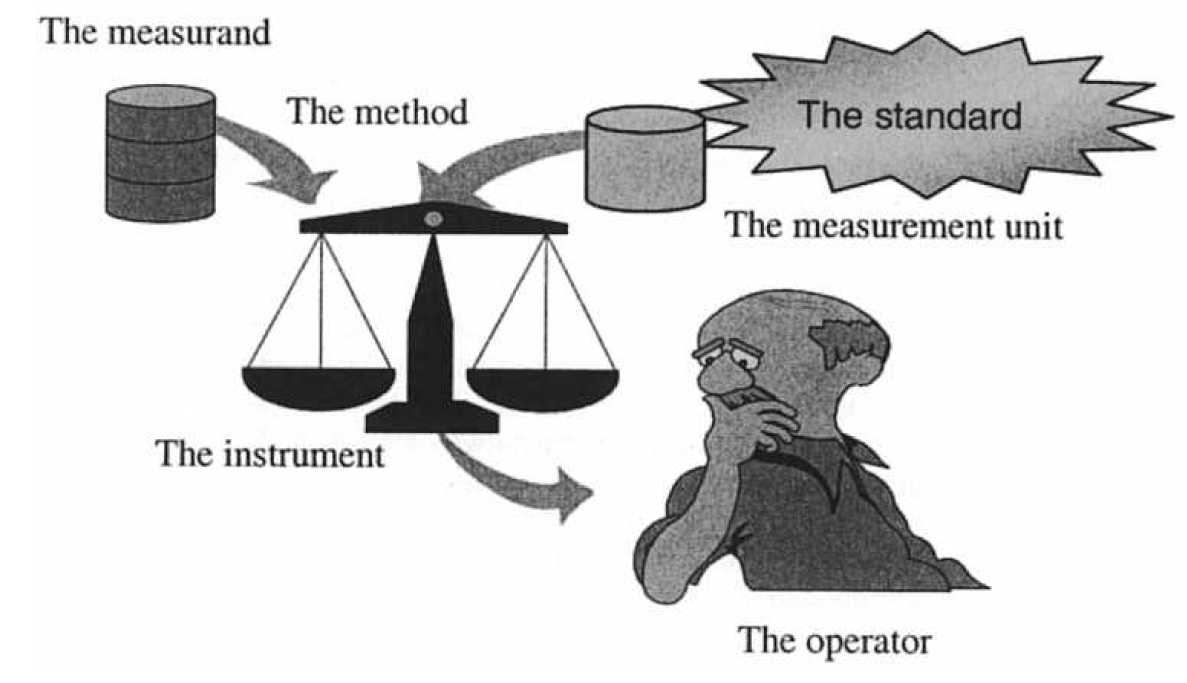
\includegraphics[scale=.5]{./img/measurement.png}
\end{figure}

  
\documentclass[12pt, right open]{memoir}
\usepackage{graphicx}
\usepackage{tikz}
\usetikzlibrary{matrix,chains,positioning,decorations.pathreplacing,arrows,automata}
\usetikzlibrary{shapes.geometric, calc, intersections}
\usepackage{mathtools}
\usepackage{amsmath}
\usepackage{float}
\floatstyle{boxed}
\restylefloat{figure}
\usepackage{multirow} %for tables
\usepackage{ifthen}
\setcounter{secnumdepth}{5}

%To reduce vetical line spaces between list items
\usepackage{enumitem}
\setlist{nolistsep,leftmargin=*}

\newcommand{\specialcell}[2][c]{%
  \begin{tabular}[#1]{@{}c@{}}#2\end{tabular}}
%  Foo bar & \specialcell{Foo\\bar} & Foo bar \\    % vertically centered
%Foo bar & \specialcell[t]{Foo\\bar} & Foo bar \\ % aligned with top rule
%Foo bar & \specialcell[b]{Foo\\bar} & Foo bar \\ % aligned with bottom rule

\newcommand{\matplus}{
~~
  }

\begin{document}

%http://www.comp.leeds.ac.uk/ai23/reading/Hopfield.pdf

% >>>>>>>> Tikz Style sheet
\tikzstyle{every pin edge}=[<-,shorten <=1pt]
\tikzstyle{neuron}=[circle,fill=black!25,minimum size=17pt,inner sep=0pt]
\tikzstyle{input neuron}=[neuron, fill=black!50]
\tikzstyle{output neuron}=[neuron, fill=black!50]
\tikzstyle{hidden neuron}=[neuron, fill=black!50]
\tikzstyle{annot} = [text width=4em, text centered]

\tikzstyle{startstop} = [rectangle, rounded corners, minimum width=3cm, minimum height=1cm,text centered, draw=black]
\tikzstyle{io} = [trapezium, trapezium left angle=70, trapezium right angle=110, minimum width=3cm, minimum height=1cm, text centered, draw=black]
\tikzstyle{process} = [rectangle, minimum width=3cm, minimum height=1cm, text centered, text width=3cm, draw=black]
\tikzstyle{decision} = [diamond, minimum width=3cm, minimum height=1cm, text centered, draw=black]
\tikzstyle{arrow} = [thick,->,>=stealth]
% <<<<<<<< Tikz Style sheet

%%%%%%%%%%%%%%%%%%%%%%%%%%%%%%%%%%%%%%%%%%%%%%%%%%%%%%%%%%%%%%%%%%%%%%%%%%%%%%%%%%%%%%%%%%%
\chapter{Common Terms to Start with Neural Network}
\section{Neural Network}
A neural network is a massively parallel distributed processor made up of simple processing units, which has a natural propensity for storing experimental knowledge and making it available for use. It resembles the brain in two aspects:
\begin{enumerate}
\item Knowledge is acquired by the network from its environment through a learning process.
\item Inter-neuron connections strengths, known as synaptic weights, are used to store the acquired knowledge. 
\end{enumerate} 
\section{Stability for a Neural Network}
Stability refers to such convergence that facilitates an end to the iterative
process. For example, if any two consecutive cycles result in the same output
for the network, then there may be no need to do more iterations. In this case,
convergence has occurred, and the network has stabilized in its operation. If
weights are being modified after each cycle, then convergence of weights
would constitute stability for the network.
In some situations, it takes many more iterations than you desire, to have
output in two consecutive cycles to be the same. Then a tolerance level on the
convergence criterion can be used. With a tolerance level, you accomplish
early but satisfactory termination of the operation of the network.

\section{Plasticity for a Neural Network}
Suppose a network is trained to learn some patterns, and in this process the
weights are adjusted according to an algorithm. After learning these patterns
and encountering a new pattern, the network may modify the weights in order
to learn the new pattern. But what if the new weight structure is not responsive
to the new pattern? Then the network does not possess plasticity—the ability
to deal satisfactorily with new short-term memory (STM) while retaining
long-term memory (LTM). Attempts to endow a network with plasticity may
have some adverse effects on the stability of your network.

Plasticity permits the developing nervous system to adapt to its surrounding environment.
\section{Short-Term Memory and Long-Term Memory}
We alluded to short-term memory (STM) and long-term memory (LTM) in the
previous paragraph. STM is basically the information that is currently and
perhaps temporarily being processed. It is manifested in the patterns that the
network encounters. LTM, on the other hand, is information that is already
stored and is not being currently processed. In a neural network, STM isusually characterized by patterns and LTM is characterized by the
connections’ weights. The weights determine how an input is processed in the
network to yield output. During the cycles of operation of a network, the
weights may change. After convergence, they represent LTM, as the weight
levels achieved are stable.

\section{Generalization}
It refers to the ability of neural networks to produce reasonable outputs for inputs not encountered during the training.

\section{Learning Algorithm}
The procedure used to perform the learning process is called a learning algorithm, the function of which is to modify the synaptic weights of the network in an orderly fashion to attain the design objective.

\end{document}
\section{Neural Processing}
How do you recognize a face in a crowd? How does an economist predict the
direction of interest rates? Faced with problems like these, the human brain
uses a web of interconnected processing elements called neurons to process
information. Each neuron is autonomous and independent; it does its work
asynchronously, that is, without any synchronization to other events taking
place. The two problems posed, namely recognizing a face and forecasting
interest rates, have two important characteristics that distinguish them from
other problems: First, the problems are complex, that is, you can’t devise a
simple step-by-step algorithm or precise formula to give you an answer; and
second, the data provided to resolve the problems is equally complex and may
be noisy or incomplete. You could have forgotten your glasses when you’re
trying to recognize that face. The economist may have at his or her disposal
thousands of pieces of data that may or may not be relevant to his or her
forecast on the economy and on interest rates. \\*
The vast processing power inherent in biological neural structures has inspired
the study of the structure itself for hints on organizing human-made computing
structures. Artificial neural networks, the subject of this book, covers the way
to organize synthetic neurons to solve the same kind of difficult, complex
problems in a similar manner as we think the human brain may. This chapter
will give you a sampling of the terms and nomenclature used to talk about
neural networks. These terms will be covered in more depth in the chapters to
follow.

\chapter{Types of Networks}

%\newcommand{\itab}[1]{\hspace{0em}\rlap{#1}}
%\newcommand{\tab} [1]{\hspace{.2\textwidth}\rlap{#1}}

The models that we overview in this chapter are the \\

\begin{enumerate}
\item Perceptron
\item Hopfield
\item Adaline
\item Feed-Forward Backpropagation
\item Bidirectional Associative Memory
\item Brain-State-in-a-Box
\item Neocognitron
\item Fuzzy Associative Memory
\item ART1
\item ART2
\end{enumerate}


%Sub heading in the chapter
\section{Based on Learning}

A network can be subject to supervised or unsupervised learning. The learning would be supervised if external criteria are used and matched by the network output, and if not, the learning is unsupervised. This is one broad way to divide different neural network approaches. Unsupervised approaches are also termed self-organizing. There is more interaction between neurons, typically with feedback and intralayer connections between neurons promoting self-organization. \\*
Supervised networks are a little more straightforward to conceptualize than unsupervised networks. You apply the inputs to the supervised network along with an expected response, much like the Pavlovian conditioned stimulus and response regimen. You mold the network with stimulus-response pairs. Astock market forecaster may present economic data (the stimulus) along with metrics of stock market performance (the response) to the neural network to the present and attempt to predict the future once training is complete. \\*
You provide unsupervised networks with only stimulus. You may, for example, want an unsupervised network to correctly classify parts from a conveyor belt into part numbers, providing an image of each part to do the classification (the stimulus). The unsupervised network in this case would act like a look-up memory that is indexed by its contents, or a Content-Addressable-Memory (CAM). \\*

\tikzstyle{rectangular_box} = [rectangle, minimum width=3cm, minimum height=1cm, text centered, text width=3cm, draw=black, fill=black!30]

%\begin{figure}[h!] 
%\centering
%\begin{tikzpicture}[node distance=2cm] 
%
%\node (learning_types) [rectangular box, xshift=8cm] {Learning};
%\node (supervised) [rectangular box, below of=learning_types, xshift=2cm] {Supervised};
%\node (unsupervised) [rectangular box, left of=supervised, xshift=8cm] {UnSupervised};
%
%\end{tikzpicture}
%\end{figure}


\chapter{External Exploration}


\section{Organizations}
Below of some of the organizations which are having major impact on Neural Network research.

\begin{itemize}
\item IEEE Neural Network Council, 
\item The INNS - International Neural Network Society
\item The ENNS - European Neural Network Society
(the most re-known and largest international scientific/technological non-profit associations
concerned with neural networks).
\item AIIA - Italian Association for Artificial Intelligence, SIREN - Italian Association for Neural Networks,
\item UNIMI-DTI - University of Milan: Department of Information Technologies.
\end{itemize}
       
\chapter{What is Perceptron?}
In machine learning, the perceptron is an algorithm for supervised classification of an input into one of several possible non-binary outputs. It is a type of linear classifier, i.e. a classification algorithm that makes its predictions based on a linear predictor function combining a set of weights with the feature vector. The algorithm allows for online learning, in that it processes elements in the training set one at a time.

The perceptron algorithm dates back to the late 1950s; its first implementation, in custom hardware, was one of the first artificial neural networks to be produced.

\section{A Bit of History}
The perceptron algorithm was invented in 1957 at the Cornell Aeronautical Laboratory by Frank Rosenblatt, funded by the United States Office of Naval Research. \hfill \\

More on the web!

\section{Definition}
In the modern sense, the perceptron is an algorithm for learning a \textbf{binary classifier}: a function that maps its input x (a real-valued vector) to an output value f(x) (a single binary value):

\[ f(x) = \left\{ 
               \begin{array}{l l}
                1  : & \quad w.x+b > 0 \\
                0  : & \quad otherwise
               \end{array} 
       \right.
\]

where...
\begin{itemize}
%\itemsep0em 
\item $\mathbf{w}$ is a vector of real-valued weights, 
\item $\mathbf{w \cdot x}$ is the dot product (which here computes a weighted sum), and $\mathbf{b}$ is the 'bias', 
\item a constant term that does not depend on any input value.
\end{itemize}

If $b$ is negative, then the weighted combination of inputs must produce a positive value greater than $|b|$ in order to push the classifier neuron over the 0 threshold. Spatially, the bias alters the position (though not the orientation) of the decision boundary. The perceptron learning algorithm does not terminate if the learning set is not linearly separable. If the vectors are not linearly separable learning will never reach a point where all vectors are classified properly. The most famous example of the perceptron's inability to solve problems with linearly nonseparable vectors is the Boolean exclusive-or problem.

In the context of neural networks, a perceptron is an \textbf{artificial neuron} using the \textbf{Heaviside step function} as the activation function. The perceptron algorithm is also termed the \textbf{single-layer perceptron}, to distinguish it from a multilayer perceptron, which is a misnomer for a more complicated neural network. As a linear classifier, the single-layer perceptron is the \textbf{simplest feedforward neural network}.

\section{Learning Algorithm}
Below is an example of a learning algorithm for a (single-layer) perceptron. For multilayer perceptrons, where a hidden layer exists, more sophisticated algorithms such as \textbf{backpropagation} must be used. Alternatively, methods such as the \textbf{delta rule} can be used if the function is \textbf{non-linear} and \textbf{differentiable}, although the one below will work as well.

When multiple perceptrons are combined in an artificial neural network, each output neuron operates independently of all the others; thus, learning each output can be considered in isolation.

\subsubsection{Definition}
We first define some variables:
\begin{itemize}
\item $y = f(\vec{\mathbf{z}})$ \, denotes the output from the perceptron for an input vector $\vec{\mathbf{z}}$.
\item $\mathbf{b}$ \, is the bias term, which in the example below we take to be 0.
\item $D = \{\vec{\mathbf{X}}_1,d_1)$,$\dots$,$(\vec{\mathbf{X}}_s,d_s)\}$ \, is the training set of s samples, where:
\begin{itemize}
\item $\vec{\mathbf{X}}_j$ is the n-dimensional input vector.
\item $\mathbf{d_j}$ \, is the desired output value of the perceptron for that input. \hfill \\
\end{itemize}

We show the values of the features as follows:
\item $x_{j,i}$ \, is the value of the ith feature of the jth training input vector.
\item $x_{j,0} = 1$ \,. 

\hfill \\ To represent the weights:
\item $w_i$ \, is the $i$th value in the weight vector, to be multiplied by the value of the $i$th input feature.
\item Because $x_{j,0}$ = 1 \,, the $w_0$ \, is effectively a learned bias that we use instead of the bias constant $b$.

\hfill \\ To show the time-dependence of $\mathbf{w}$, we use:
\item $w_i(t)$ \, is the weight $i$ at time $t$.
\item $\alpha$ \, is the learning rate, where $0 < \alpha \leq 1$.

Too high a learning rate makes the perceptron periodically oscillate around the solution unless additional steps are taken.
\end{itemize}

\subsection{Steps}

\begin{enumerate}

\item Initialise the weights and the threshold. Weights may be initialised to $0$ or to a small random value. In the example below, we use $0$.

\item  For each example $j$ \, in our training set $D$ \,, perform the following steps over the input $\mathbf{x}_j$\, and desired output $d_j$ \,:

\begin{enumerate}
\item Calculate the actual output: \hfill \\
$\mathbf{y_j(t) = f[\mathbf{w}(t)\cdot\mathbf{x}_j] = f[w_0(t) + w_1(t)x_{j,1} + w_2(t)x_{j,2} + \dotsb + w_n(t)x_{j,n}]}$
\item Update the weights: \hfill \\
$\mathbf{w_i(t+1) = w_i(t) + \alpha (d_j - y_j(t)) x_{j,i}}$ \, for all feature $\mathbf{0 \leq i \leq n}$.
\end{enumerate}

\item  For offline learning, the step 2 may be repeated until the iteration error 
$\mathbf{\frac{1}{s} \sum_{j=1}^s |d_j - y_j(t)|}$ \, is less than a user-specified error threshold $\mathbf{\gamma}$\,, or a predetermined number of iterations have been completed.

\end{enumerate}

The algorithm updates the weights after steps $2a$ and $2b$. These weights are immediately applied to a pair in the training set, and subsequently updated, rather than waiting until all pairs in the training set have undergone these steps.

\section{Convergence}
The perceptron is a linear classifier, therefore it will never get to the state with all the input vectors classified correctly if the training set $\mathbf{D}$ is not linearly separable, i.e. if the positive examples can not be separated from the negative examples by a hyperplane.

\section{Pocket Algorithm}
The pocket algorithm with ratchet (Gallant, 1990) solves the stability problem of perceptron learning by keeping the best solution seen so far "in its pocket". The pocket algorithm then returns the solution in the pocket, rather than the last solution. It can be used also for non-separable data sets, where the aim is to find a perceptron with a small number of misclassifications.


\section{Example}
A perceptron learns to perform a binary NAND function on inputs $x_1$ \, and $x_2$ \,.

\begin{itemize}
\item Inputs: $x_0$ \,, $x_1$ \,, $x_2$ \,, with input $x_0$ \, held constant at 1.
\item Threshold ($\theta$): $0.5$
\item Bias ($b$): 0
\item Learning rate ($r$): 0.1
\item Training set, consisting of four samples: $\{((1, 0, 0), 1), ((1, 0, 1), 1), ((1, 1, 0), 1), ((1, 1, 1), 0)\}$ \,
\end{itemize}


In the following, the final weights of one iteration become the initial weights of the next. Each cycle over all the samples in the training set is demarcated with heavy lines.

%For time being we will capture the image from wiki and put it here!

%\begin{center}
%
%\begin{table}[ht]
%\caption{Example of weight updates for the Perceptron Network}
%\label{tab:example_of_weight_update_for_the_perceptron_network}
%%\resizebox{\textwidth}{!}
%
%\begin{tabular}{|l|*{17}{c|}}
%\hline
%\multicolumn{2}{|c|} {I/P} & \specialcell{Intial\\Weights} & \multicolumn{3}{|c|}{O/P} & Error & Correction & Final Weights \\
%\hline
%\specialcell{Sensor\\Values} & \specialcell{Desired\\O/P} &  & Per sensor  & Sum & Network & & & \\
%\hline
%\multicolumn{3}{|c|} $x_0$ & $x_1$ & $x_2$ & $z$ & $w_0$ & $w_1$ & $w_2$ & $c_0$ & $c_1$ & $c_2$ & $s$ & $n$ & $e$ & $d$ & $w_0$ & $w_1$ & $w_2$ \\
%\hline
%\end{tabular}
%
%\end{table}
%
%\end{center}

\begin{figure}
\caption{Example of weight updates for the Perceptron Network}
\label{tab:example_of_weight_update_for_the_perceptron_network}
\centering
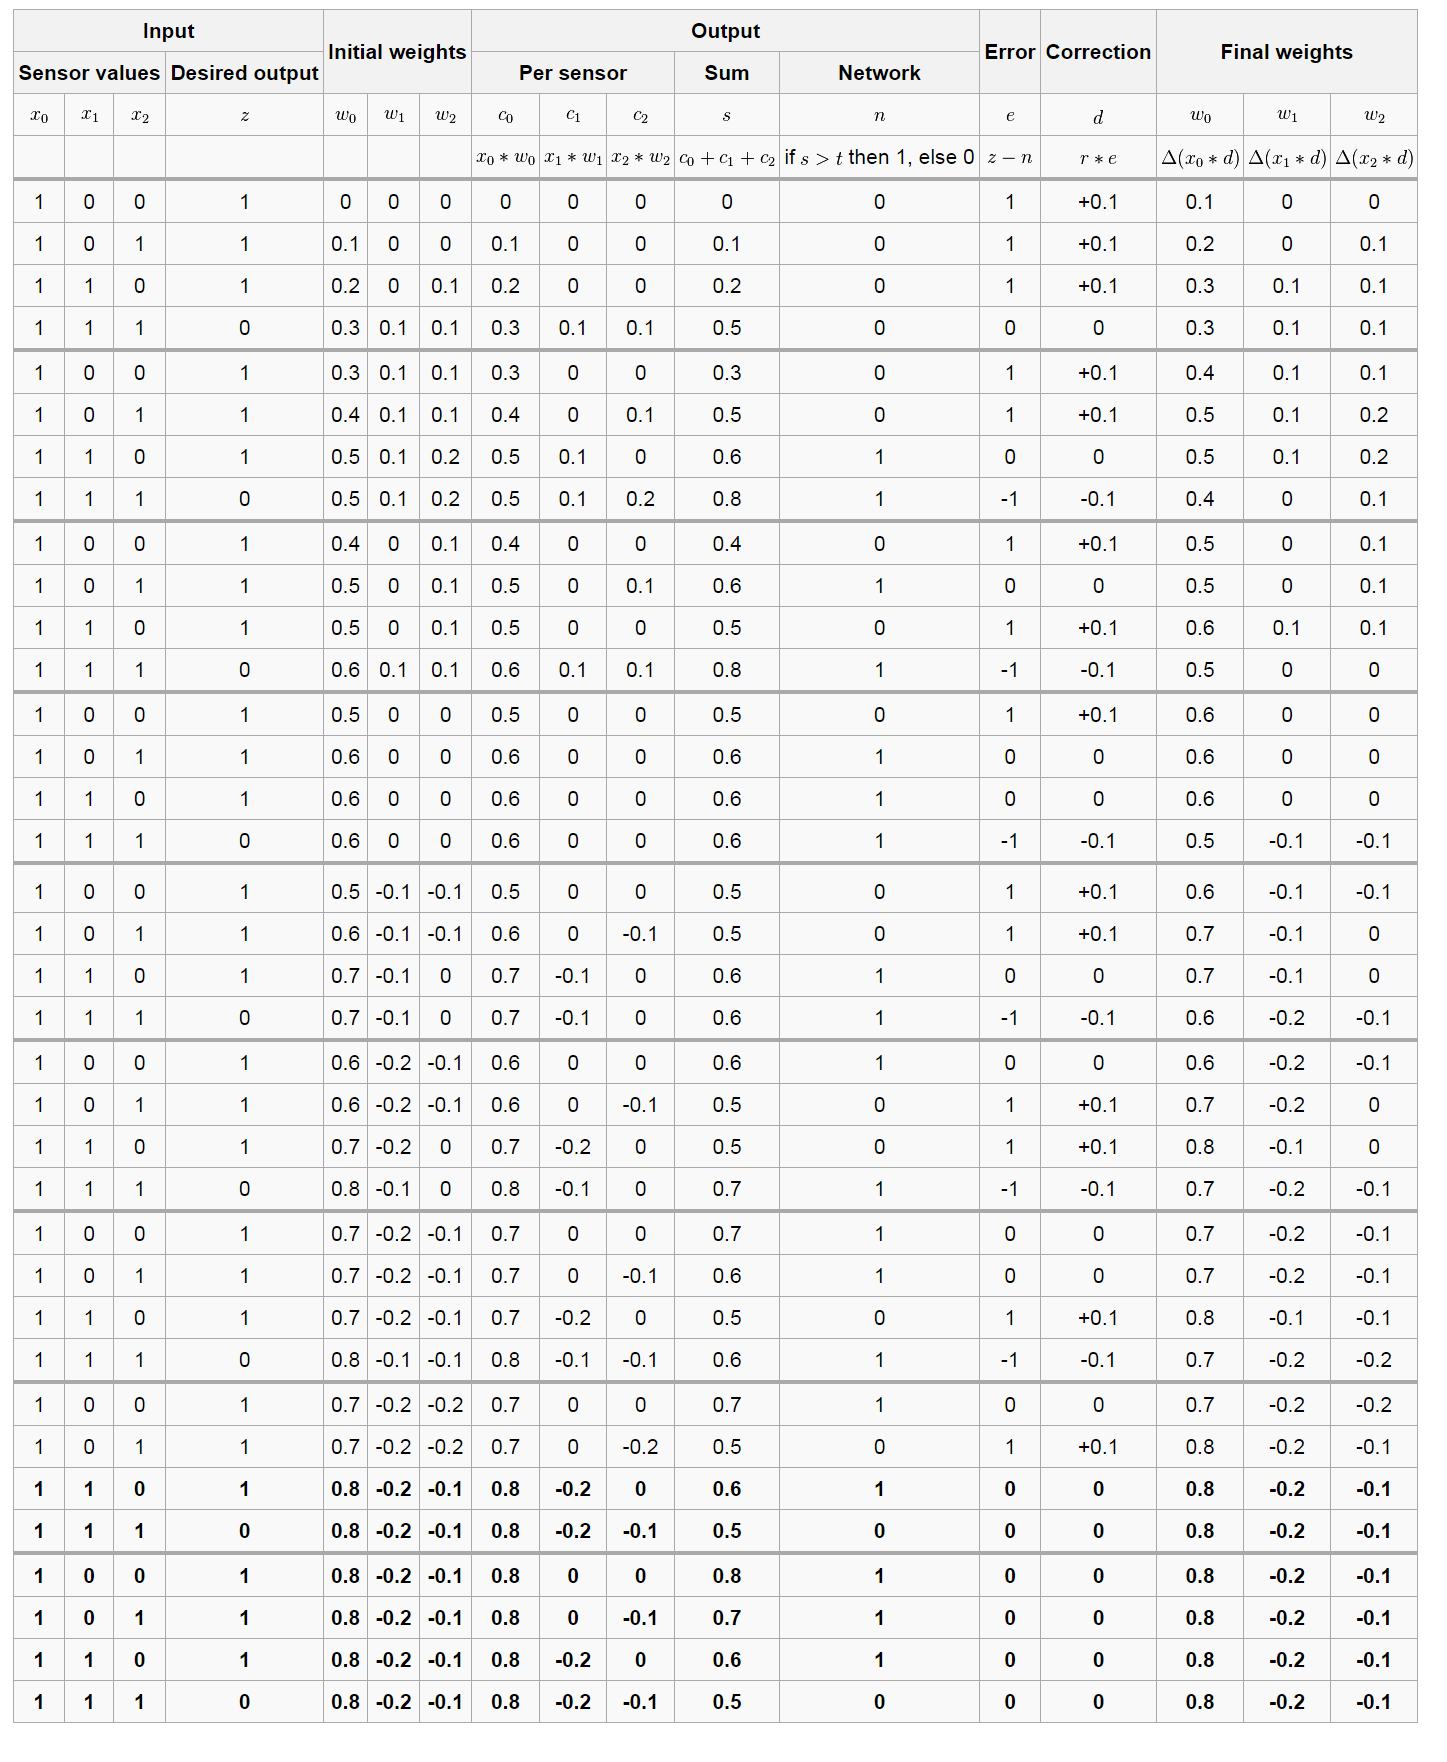
\includegraphics[scale=.5]{./img/example_weight_updates_perceptron_network.png}
\end{figure}

\section{Example : $aja/example/ann/perceptron\_network.cpp$}


In our C++ implementation of this network, we have the following classes: we have separate classes for input neurons and output neurons. The \textbf{input\_neuron} class is for the input neurons. This class has weight and activation as data members. The \textbf{output\_neuron} class is similar and is for the output neuron. It is declared as a friend class in the \textbf{input\_neuron} class. The output neuron class has also a data member called output. There is a network class, which is a friend class in the \textbf{output\_neuron} class. An instance of the network class is created with four input neurons. These four neurons are all connected with one output neuron.

\subsubsection{input\_neuron class}
The member functions of the input\_neuron class are: 
\begin{itemize}
\item A default constructor, 
\item A second constructor that takes a real number as an argument, and 
\item A function that calculates the output of the input neuron. \\
\end{itemize}


The constructor taking one argument uses that argument to set the value of the weight on the connection between the input neuron and the output neuron. The functions that determine the neuron activations and the network output are declared public. The activations of the neurons are calculated with functions defined in the neuron classes. A threshold value is used by a member function of the output neuron to determine if the neuron’s activation is
large enough for it to fire, giving an output of 1.

\subsubsection{Implementation of Functions}


The network is designed to have four neurons in the input layer. Each of them is an object of class input\_neuron, and these are member classes in the class network. There is one explicitly defined output neuron of the class out\_neuron. The network constructor also invokes the neuron constructor for each input layer neuron in the network by providing it with the initial weight for its connection to the neuron in the output layer. The constructor for the output neuron is also invoked by the network constructor, at the same time initializing the output and activation data members of the output neuron each to zero. To make sure there is access to needed information and functions, the output neuron is declared a friend class in the class input\_neuron. The network is declared as a friend class in the class out\_neuron.

\subsubsection{Input/Output}
There are two data files used in this program. One is for setting up the weights, and the other for setting up the input vectors. On the command line, you enter the program name followed by the weight file name and the input file name. 
You can find a file called weight.dat, which contains the following data: \\
2.0 3.0 3.0 2.0 \\
3.0 0.0 6.0 2.0 \\
These are two weight vectors. \\
You can find a file called input.dat with the two data vectors below: \\
1.95 0.27 0.69 1.25 \\
0.30 1.05 0.75 0.19 \\

\subsection{Execution}
\begin{lstlisting}[caption={perceptron\_netwotk.cpp output}] %language=C++, 
example/ann/perceptron_network example/ann/weight.dat example/ann/input.dat

This program is for a perceptron network with  
input layer of 4 neurons, each connected to the 
output neuron.

This example takes Real number as Input Signals
Please enter the number of weights/vectors : 2
This is vector # 1
Please enter a threshold value for 
output neuron, eg 7.0 : 7

Input neuron 1 value is : 1.95 weight is : 2  
and its activation is : 3.9
Input neuron 2 value is : 0.27 weight is : 3  
and its activation is : 0.81
Input neuron 3 value is : 0.69 weight is : 3  
and its activation is : 2.07
Input neuron 4 value is : 1.25 weight is : 2  
and its activation is : 2.5

Output neuron activation is : 9.28

The output neuron activation exceeds the-
threshold value of 7
Output value is 1

This is vector # 2
Please enter a threshold value for 
output neuron, eg 7.0 : 7

Input neuron 1 value is : 0.3 weight is : 3  
and its activation is : 0.9
Input neuron 2 value is : 1.05 weight is : 0  
and its activation is : 0
Input neuron 3 value is : 0.75 weight is : 6  
and its activation is : 4.5
Input neuron 4 value is : 0.19 weight is : 2  
and its activation is : 0.38

Output neuron activation is : 5.78

The output neuron activation is smaller than the- 
threshold value of 7
Output value is 0
\end{lstlisting}


\chapter{XOR Function}
The ability of a Perceptron in evaluating functions was brought into question
when Minsky and Papert proved that a simple function like XOR (the logical
function exclusive or) could not be correctly evaluated by a Perceptron. The
XOR logical function, f(A,B), is as follows: \\

\begin{table} 
\caption{XOR Table}
\label{tab:xor_table}
\begin{tabular}{|l|l|c|}
\hline
A & B & $f(A,b) = XOR(A,B)$ \\
\hline
0 & 0 & 0 \\ 
\hline
0 & 1 & 1 \\ 
\hline
1 & 0 & 1 \\ 
\hline
1 & 1 & 0 \\ 
\hline
\end{tabular}
\end{table}

Minsky and Papert showed that it is impossible to come up with the proper set of weights for the neurons in the single layer of a simple Perceptron to evaluate the XOR function. The reason for this is that such a Perceptron, one with a single layer of neurons, requires the function to be evaluated, to be linearly separable by means of the function values. The concept of \textbf{linear separability} is explained next. But let us show you first why the simple perceptron fails to compute this function.

Since there are two arguments for the XOR function, there would be two
neurons in the input layer, and since the function’s value is one number, there would be one output neuron. Therefore, you need two weights w 1 and w 2 ,and a threshold value  ̧. Let us now look at the conditions to be satisfied by the w’s and the  ̧ so that the outputs corresponding to given inputs would be as for the XOR function.First the output should be 0 if inputs are 0 and 0. The activation works out as 0. To get an output of 0, you need 0 <  ̧. This is your first condition. \ref{tab:conditions_on_weights} shows this and two other conditions you need, and why.

\begin{table} 
\caption{Conditions on Weights}
\label{tab:conditions_on_weights}
\begin{tabular}{|l|l|c|c|}
\hline
Input & Activation & Output & Needed Condition  \\
\hline
0, 0  & 0          & 0      & 0 <               \\ 
\hline
0, 1  & $w_1$      & 1      & $w_1$ >           \\ 
\hline
1, 0  & $w_2$      & 1      & $w_2$ <            \\ 
\hline
1, 1  & $w_1 + w_2$ & 0      & $w_1 + w_2$ <       \\ 
\hline
\end{tabular}
\end{table}

From the first three conditions, you can deduce that the sum of the two weights has to be greater than  ̧, which has to be positive itself. Line 4 is inconsistent with lines 1, 2, and 3, since line 4 requires the sum of the two weights to be less than, This affirms the contention that it is not possible to compute the XOR function with a simple perceptron.

Geometrically, the reason for this failure is that the inputs (0, 1) and (1, 0) with which you want output 1, are situated diagonally opposite each other, when plotted as points in the plane, as shown below in a diagram of the output (1=T,0=F): \\

\begin{tabular}{|c|c|}
\hline
F & T \\ \hline
T & F \\ \hline
\end{tabular}

You can’t separate the T’s and the F’s with a straight line. This means that you cannot draw a line in the plane in such a way that neither (1, 1) ->F nor (0,0)->F is on the same side of the line as (0, 1) ->T and (1, 0)-> T.

\section{Linear Separability}
What linearly separable means is, that a type of a linear barrier or a
separator \textbf{a line in the plane}, or \textbf{a plane in the three-dimensional space}, or \textbf{a hyperplane in higher dimensions} should exist, so that the set of inputs that give rise to one value for the function all lie on one side of this barrier, while on the other side lie the inputs that do not yield that value for the function. A hyperplane is a surface in a higher dimension, but with a linear equation defining it much the same way a line in the plane and a plane in the three-dimensional space are defined.

To make the concept a little bit clearer, consider a problem that is similar but, let us emphasize, not the same as the XOR problem.

\newcommand{\Depth}{4}
\newcommand{\Height}{4}
\newcommand{\Width}{4}
\begin{figure}
\centering
\caption{Separating plane}
\label{fig:separating_plane}
\begin{tikzpicture}
\coordinate (O) at (0,0,0);
\coordinate (A) at (0,\Width,0);
\coordinate (B) at (0,\Width,\Height);
\coordinate (C) at (0,0,\Height);
\coordinate (D) at (\Depth,0,0);
\coordinate (E) at (\Depth,\Width,0);
\coordinate (F) at (\Depth,\Width,\Height);
\coordinate (G) at (\Depth,0,\Height);

\coordinate (1) at (\Depth/2, 0, 0);
\coordinate (2) at (\Depth/2, 0, \Height);
\coordinate (3) at (\Depth/2, \Width, 0);
\coordinate (4) at (\Depth/2, \Width, \Height);

\draw[blue,fill=yellow!80] (O) -- (C) -- (G) -- (D) -- cycle;% Bottom Face
\draw[blue,fill=blue!30] (O) -- (A) -- (E) -- (D) -- cycle;% Back Face
\draw[blue,fill=red!10] (O) -- (A) -- (B) -- (C) -- cycle;% Left Face
\draw[blue,fill=red!20,opacity=0.8] (D) -- (E) -- (F) -- (G) -- cycle;% Right Face
\draw[blue,fill=red!20,opacity=0.6] (C) -- (B) -- (F) -- (G) -- cycle;% Front Face
\draw[blue,fill=red!20,opacity=0.8] (A) -- (B) -- (F) -- (E) -- cycle;% Top Face
%\draw[green,fill=red!20,opacity=0.8] (1) -- (2) -- (3) -- (4) % ToDo: Centre line
% Following is for debugging purposes so you can see where the points are
% These are last so that they show up on top
\foreach \xy in {O, A, B, C, D, E, F, G}{
    \node at (\xy) {\xy};
}
\end{tikzpicture}
\end{figure}

Imagine a cube of 1-unit length for each of its edges and lying in the positive octant in a xyz-rectangular coordinate system with one corner at the origin.
The other corners or vertices are at points with coordinates (0, 0, 1), (0, 1, 0),(0, 1, 1), (1, 0, 0), (1, 0, 1), (1, 1, 0), and (1, 1, 1). Call the origin O, and the seven points listed as C, A, B, D, G, E, and F, respectively. Then any two faces
opposite to each other are linearly separable because you can define theseparating plane as the plane halfway between these two faces and also parallel to these two faces.
For example, consider the faces defined by the set of points O, A, B, and C and
by the set of points D, E, F, and G. They are parallel and 1 unit apart, as you
can see in Figure 5.1. The separating plane for these two faces can be seen to
be one of many possible planes—any plane in between them and parallel to
them. One example, for simplicity, is the plane that passes through the points
(1/2, 0, 0), (1/2, 0, 1), (1/2, 1, 0), and (1/2, 1, 1). Of course, you need only
specify three of those four points because a plane is uniquely determined by
three points that are not all on the same line. So if the first set of points
corresponds to a value of say, +1 for the function, and the second set to a value
of –1, then a single-layer Perceptron can determine, through some training
algorithm, the correct weights for the connections, even if you start with the
weights being initially all 0

Consider the set of points O, A, F, and G. This set of points cannot be linearly
separated from the other vertices of the cube. In this case, it would be
impossible for the single-layer Perceptron to determine the proper weights for
the neurons in evaluating the type of function we have been discussing.
\chapter{References}
Without following links Ctrl + c and Ctrl + v would have not happened!

http://en.wikipedia.org/wiki/Perceptron

              
\chapter{Pros and Cons of Artificial Neural Network}
\section{Benefits}





\part{Apache Spark}
%Relative path from root diectory

\section{Spark MLLib Linear Model Class Internals}
 
RegressionModel
GeneralizedLinearModel
LinearRegressionModel
LinearRegressionWithSGD


%Ref: http://get-software.net/graphics/pgf/contrib/pgf-umlcd/pgf-umlcd-manual.pdf (not used)
%\begin{tikzpicture}
%\begin {class}[text width=8cm]{ClassName}{0 ,0}
%\attribute{name : attribute type}
%\attribute{name : attribute type = default value}
%\operation{name ( parameter list ) : type of valuereturned}
%% virtual operation
%\operation[0]{ name ( parameters list ) : type ofvalue returned}
%\end {class}
%\end {tikzpicture}

%Ref: tikzuml-v0.9.9.pdf
\begin{tikzpicture}
\begin{umlpackage } [ x=0,y=0]{ package−name}
\end{umlpackage }
\ umlemptyclass[width=15ex] { class20}
\ umlemptyclass[y=−2, width=30ex ] { class40}
\end{tikzpicture}

%Ref: http://get-software.net/graphics/pstricks/contrib/uml/uml.pdf

%Ref: http://www.texample.net/tikz/examples/tree/
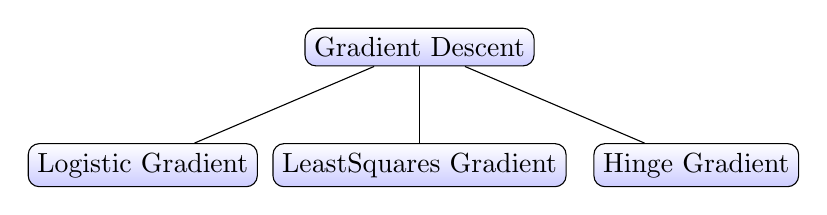
\begin{tikzpicture}[sibling distance=10em,
  every node/.style = {shape=rectangle, rounded corners,
    draw, align=center,
    top color=white, bottom color=blue!20}]]
  \node {Gradient Descent}
    child { node {Logistic Gradient} }
    child { node {LeastSquares Gradient} }
    child { node {Hinge Gradient} };
\end{tikzpicture}

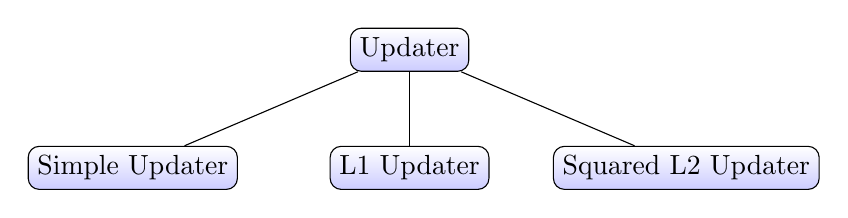
\begin{tikzpicture}[sibling distance=10em,
  every node/.style = {shape=rectangle, rounded corners,
    draw, align=center,
    top color=white, bottom color=blue!20}]]
  \node {Updater}
     child { node {Simple Updater} }
     child { node {L1 Updater} }
     child { node {Squared L2 Updater} };
\end{tikzpicture}

%Ref: UML http://ctan.imsc.res.in/graphics/pgf/contrib/pgf-umlcd/pgf-umlcd-manual.pdf

LinearRegressionWithSGD.train.run.





\end{document}
